%%%%%%%% ICML 2026 EXAMPLE LATEX SUBMISSION FILE %%%%%%%%%%%%%%%%%

\documentclass{article}


% Added by Van
\usepackage{svg}
\svgsetup{inkscapelatex=false}
\usepackage{float}
\usepackage{placeins}
% Preamble
\usepackage[most]{tcolorbox}

\newtcolorbox{positionbox}{
  enhanced,
  colback=white,
  colframe=black,
  boxrule=0.8pt,
  sharp corners,
  left=1em,
  right=1em,
  top=0.5em,
  bottom=0.5em,
  before skip=1.2em,
  after skip=1.2em,
  title=Our position,
  coltitle=white,
  fonttitle=\bfseries,
  colbacktitle=black,
  attach boxed title to top left={xshift=0pt,yshift=0pt},
  boxed title style={
    sharp corners,
    boxrule=0pt,
    colback=black,
    width=\linewidth,
    left=0.5em,
    top=0.15em,
    bottom=0.15em
  }
}

% Preamble
\definecolor{feedbackblue}{HTML}{EEF7FF}
\definecolor{feedbackline}{HTML}{5B9BD5}
\definecolor{feedbacktext}{HTML}{1F3A5F}

\newtcolorbox{feedbackbox}{
  enhanced,
  colback=feedbackblue,
  colframe=feedbackline,
  boxrule=0pt,
  leftrule=4pt,
  arc=2pt,
  left=0.9em,
  right=0.9em,
  top=0.6em,
  bottom=0.6em,
  before skip=1em,
  after skip=1em,
  fontupper=\small\color{feedbacktext}
}

% Added by Sam
\usepackage{tcolorbox}

% Added by charlie
\usepackage{listings}



% ====================================
% --------- ANGELO'S ADD-ONS ---------
% ====================================
% For theorems and such
\usepackage{amsmath}
\usepackage{amssymb}% http://ctan.org/pkg/amssymb
\usepackage{mathtools}
\usepackage{amsthm}
\usepackage{epigraph} % in preamble

\usepackage{xcolor}
\newtheorem{example}{Example}
% For tables with multi-row cells
\usepackage{multirow}
\usepackage[inline]{enumitem}

\usepackage{xurl}

%%%%%%%%%%%%%%%%%%%%%%%%%%%%%%%%
% THEOREMS
% %%%%%%%%%%%%%%%%%%%%%%%%%%%%%%%%
% \theoremstyle{plain}
% \newtheorem{theorem}{Theorem}[section]
% \newtheorem{proposition}[theorem]{Proposition}
% \newtheorem{lemma}[theorem]{Lemma}
% \newtheorem{corollary}[theorem]{Corollary}
% \theoremstyle{definition}
% \newtheorem{definition}[theorem]{Definition}
% \newtheorem{assumption}[theorem]{Assumption}
% \theoremstyle{remark}
% \newtheorem{remark}[theorem]{Remark}

% Todonotes is useful during development; simply uncomment the next line
%    and comment out the line below the next line to turn off comments
%\usepackage[disable,textsize=tiny]{todonotes}
\usepackage[textsize=tiny]{todonotes}


% Recommended, but optional, packages for figures and better typesetting:
\usepackage{microtype}
\usepackage{graphicx}
\usepackage{subcaption}
\usepackage{booktabs} % for professional tables

% hyperref makes hyperlinks in the resulting PDF.
% If your build breaks (sometimes temporarily if a hyperlink spans a page)
% please comment out the following usepackage line and replace
% \usepackage{icml2026} with \usepackage[nohyperref]{icml2026} above.
\usepackage{hyperref}


% Attempt to make hyperref and algorithmic work together better:
\newcommand{\theHalgorithm}{\arabic{algorithm}}

% Use the following line for the initial blind version submitted for review:
% \usepackage{icml2026}

% For preprint, use
\usepackage[preprint]{icml2026}

% If accepted, instead use the following line for the camera-ready submission:
% \usepackage[accepted]{icml2026}

\usepackage{amsmath}
\usepackage{amssymb}
\usepackage{mathtools}
\usepackage{amsthm}

% if you use cleveref..
\usepackage[capitalize,noabbrev]{cleveref}

%%%%%%%%%%%%%%%%%%%%%%%%%%%%%%%%
% THEOREMS
%%%%%%%%%%%%%%%%%%%%%%%%%%%%%%%%
\theoremstyle{plain}
\newtheorem{theorem}{Theorem}[section]
\newtheorem{proposition}[theorem]{Proposition}
\newtheorem{lemma}[theorem]{Lemma}
\newtheorem{corollary}[theorem]{Corollary}
\theoremstyle{definition}
\newtheorem{definition}[theorem]{Definition}
\newtheorem{assumption}[theorem]{Assumption}
\theoremstyle{remark}
\newtheorem{remark}[theorem]{Remark}

% Todonotes is useful during development; simply uncomment the next line
%    and comment out the line below the next line to turn off comments
%\usepackage[disable,textsize=tiny]{todonotes}
\usepackage[textsize=tiny]{todonotes}

% The \icmltitle you define below is probably too long as a header.
% Therefore, a short form for the running title is supplied here:
\icmltitlerunning{Spotlight paper at the ICML 2026 Trustworthy AI4GOOD Workshop}




\begin{document}

\twocolumn[
  \icmltitle{Multi-Agent AI Systems Need Institutional Design,\\
  Not Just Model-Level Alignment}

  % It is OKAY to include author information, even for blind submissions: the
  % style file will automatically remove it for you unless you've provided
  % the [accepted] option to the icml2026 package.

  % List of affiliations: The first argument should be a (short) identifier you
  % will use later to specify author affiliations Academic affiliations
  % should list Department, University, City, Region, Country Industry
  % affiliations should list Company, City, Region, Country

  % You can specify symbols, otherwise they are numbered in order. Ideally, you
  % should not use this facility. Affiliations will be numbered in order of
  % appearance and this is the preferred way.
  \icmlsetsymbol{cofirst}{*}
  \icmlsetsymbol{colast}{\textdagger}

  \begin{icmlauthorlist}
    \icmlauthor{Van QT Truong}{cofirst,upenn,utor,euro}
    \icmlauthor{Xuanqiang Angelo Huang}{cofirst,utor,euro,eth,idai}
    \icmlauthor{Erivan Inan}{utor,euro}
    \icmlauthor{Ryan Faulkner}{utor,euro}
    \icmlauthor{Jo{\"e}l Naoki Christoph}{harvard}
    \icmlauthor{Terry Jingchen Zhang}{colast,utor,euro}
    %\icmlauthor{}{sch}
    \icmlauthor{David Guzman Piedrahita}{colast,utor,euro,eth}
    \icmlauthor{Zhijing Jin}{colast,utor,euro,maxp}
  \end{icmlauthorlist}

  \icmlaffiliation{upenn}{University of Pennsylvania}
  \icmlaffiliation{utor}{Jinesis Lab, University of Toronto \& Vector Institute}
  \icmlaffiliation{euro}{EuroSafeAI}
  \icmlaffiliation{eth}{ETH Z\"urich}
  \icmlaffiliation{idai}{Institute for Decentralized AI, Oxford}
  \icmlaffiliation{maxp}{Max Planck Institute for Intelligent Systems, Tübingen, Germany}
  \icmlaffiliation{harvard}{Harvard Kennedy School}

  \icmlcorrespondingauthor{Van QT Truong}{heyvan@cs.toronto.edu}
  \icmlcorrespondingauthor{Xuanqiang Angelo Huang}{hxuanqiang@ethz.ch}
  \icmlcorrespondingauthor{Zhijing Jin}{zjin@cs.toronto.edu}

  % You may provide any keywords that you find helpful for describing your
  % paper; these are used to populate the "keywords" metadata in the PDF but
  % will not be shown in the document
  \icmlkeywords{large language models (LLMs), multi-agent systems, mechanism design, AI agents}

  \vskip 0.3in
]

% this must go after the closing bracket ] following \twocolumn[ ...

% Use ONE of the following lines. DO NOT remove the command.
% If you have no special notice, KEEP empty braces:
\printAffiliationsAndNotice{
\textsuperscript{*}Equal co-first authors.
\textsuperscript{\textdagger}Equal co-last authors.} % no special notice (required even if empty)
% Or, if applicable, use the standard equal contribution text:
% \printAffiliationsAndNotice{\icmlEqualContribution}


% \textbf{Primary area:} Socio-technical aspects of AI
% \textbf{Secondary:} Language

% \textbf{Keywords:} multi-agent AI, AI agents, cooperation, institutional design, AI safety, sanctioning mechanisms, public goods games, mechanism design, agent societies}


% ====================================
% , , , , - ABSTRACT , , , , -
% The abstract must briefly state the position (e.g., “This position paper argues that <statement of the position>.”).
% ====================================
\newcommand{\ANG}[1]{
    {\color{orange} {*ANG: #1}}}
\newcommand\VAN[1]{
    {\color{blue} {VAN: #1}}}
\newcommand\vqt[1]{
    {\color{blue} {#1}}}
\newcommand\TODO[1]{
    {\color{red} {*TODO: #1}}}
\newcommand\REVISED[1]{
    {\color{purple} {#1}}}
\newcommand\ERI[1]{
    {\color{violet} {ERIVAN: #1}}}
\newcommand\RYAN[1]{
    {\color{teal} {RYAN: #1}}}
\newcommand\JOEL[1]{
    {\color{magenta} {*JOEL: #1}}}
\renewcommand{\ANG}[1]{}
\renewcommand\VAN[1]{}
\renewcommand\vqt[1]{#1}
\renewcommand\TODO[1]{}
\renewcommand\REVISED[1]{#1}
\renewcommand\ERI[1]{}
\renewcommand\RYAN[1]{}
\renewcommand\JOEL[1]{}

% Color list: https://www.overleaf.com/learn/latex/Using_colors_in_LaTeX
    
\begin{abstract}
% \section{Abstract}
Autonomous AI agents powered by large language models are increasingly embedded in multi-agent settings, where success depends on cooperation and sharing tools, finite resources, and decision authority. These shared resources form artificial commons, where well-known collective-action failures can reappear. Current alignment techniques, which primarily evaluate individual models for their appropriate responses to humans, are insufficient to address these emergent system-level dynamics.
\textbf{This position paper argues that future AI safety research should evaluate agent societies as governed systems, in addition to collections of individually aligned models.}
We use sanctions to illustrate one axis where institutional rules acquire practical consequences and reveal the broader institutional structures that shape cooperation.
We make three contributions.
\textbf{First}, we argue for evaluating the \emph{model-in-institution}, since individually aligned agents can still produce collectively harmful outcomes through agent-group interactions.
\textbf{Second}, we distinguish sanctions from the broader institutional functions that give them meaning and legitimacy.
\textbf{Third}, we propose an evaluation agenda for testing cooperation-shaping institutions across repeated multi-agent dilemmas, varying not only model family and task, but also resource structure, group composition, enforcement architecture, and repair pathways.
\textbf{Our goal is to design agent institutions that sustain \emph{beneficial} forms of cooperation, rather than simply maximizing cooperation as an end in itself.}

 % \RYAN{It may helpful to qualify the strength of our claim here. For instance are we saying that sanctions are a necessary condition for functioning agent societies? Also, do we need the following sentence about punishment?} \VAN{Done! June 29 @Ryan n @Angelo can you check now?} \RYAN{Nice, looks good to me now!}
\end{abstract}


% ====================================
% , , , - INTRODUCTION , , , , 
% ------------------------------------
% Add a clear contributions paragraph at the end of the introduction.
% The introduction must state the position, using bold text.
% ====================================

% \ANG{
% Reviewer F9S3
% > The "model-in-institution" unit of evaluation is asserted but not operationalized. What does it actually mean to evaluate a model embedded in an institution? Is the institution held fixed and the model varied, or vice versa? How are confounds between role and behavior separated? Section 5 lists candidate metrics (Table 1; Table 5 in the appendix) but does not give a methodology for designing controlled comparisons. Given that this is the central claim, it deserves more than a metrics table.

% }



\section{Introduction}


Consider two ways an autonomous agent might execute a \$10M purchase on behalf of its principal: a cryptocurrency transfer to an address, or a wire through the conventional banking system. Suppose that the agent corrupts a single character of the recipient identifier. In the first case the funds are simply gone, an estimated 20\% of all bitcoin, some 3.7 million BTC, is already permanently inaccessible through key loss and misdirected transfers \citep{LostPasswordsLock2021}\footnote{Even here the exceptions prove the rule: when losses grow large enough, ostensibly trustless communities improvise institutional repairs, as in the Ethereum DAO fork \citep{dupontExperimentsAlgorithmicGovernance2017} following a hack draining 3.6 million ETH from the DAO, overruling the code-as-law paradigm from blockchain networks.}. In the second, a web of institutions exists to prevent cascading interaction failures: when Citibank mistakenly wired \$894M of its own funds to Revlon's lenders in 2020 instead of a \$7.8M interest payment, recall notices, injunctions, and ultimately appellate restitution doctrine returned the money \citep{CitibankSues2020}. The agent's intent, and its alignment with its principal, was identical in both scenarios. What differed was the institutional setting (i.e. cryptocurrency vs. traditional banking) in which it acted.
% \VAN{TODO reword last 2 sentences here. Sounds weird and AIish}


% JULY 2 TODO = \VAN{. TODO still need to doublecheck text examples and manuscript body one final pass. Also make fig examples match the list on Latex line 330 for Tragedy of the Commons and institutional responses}
\begin{figure*}[!t]
    \centering
    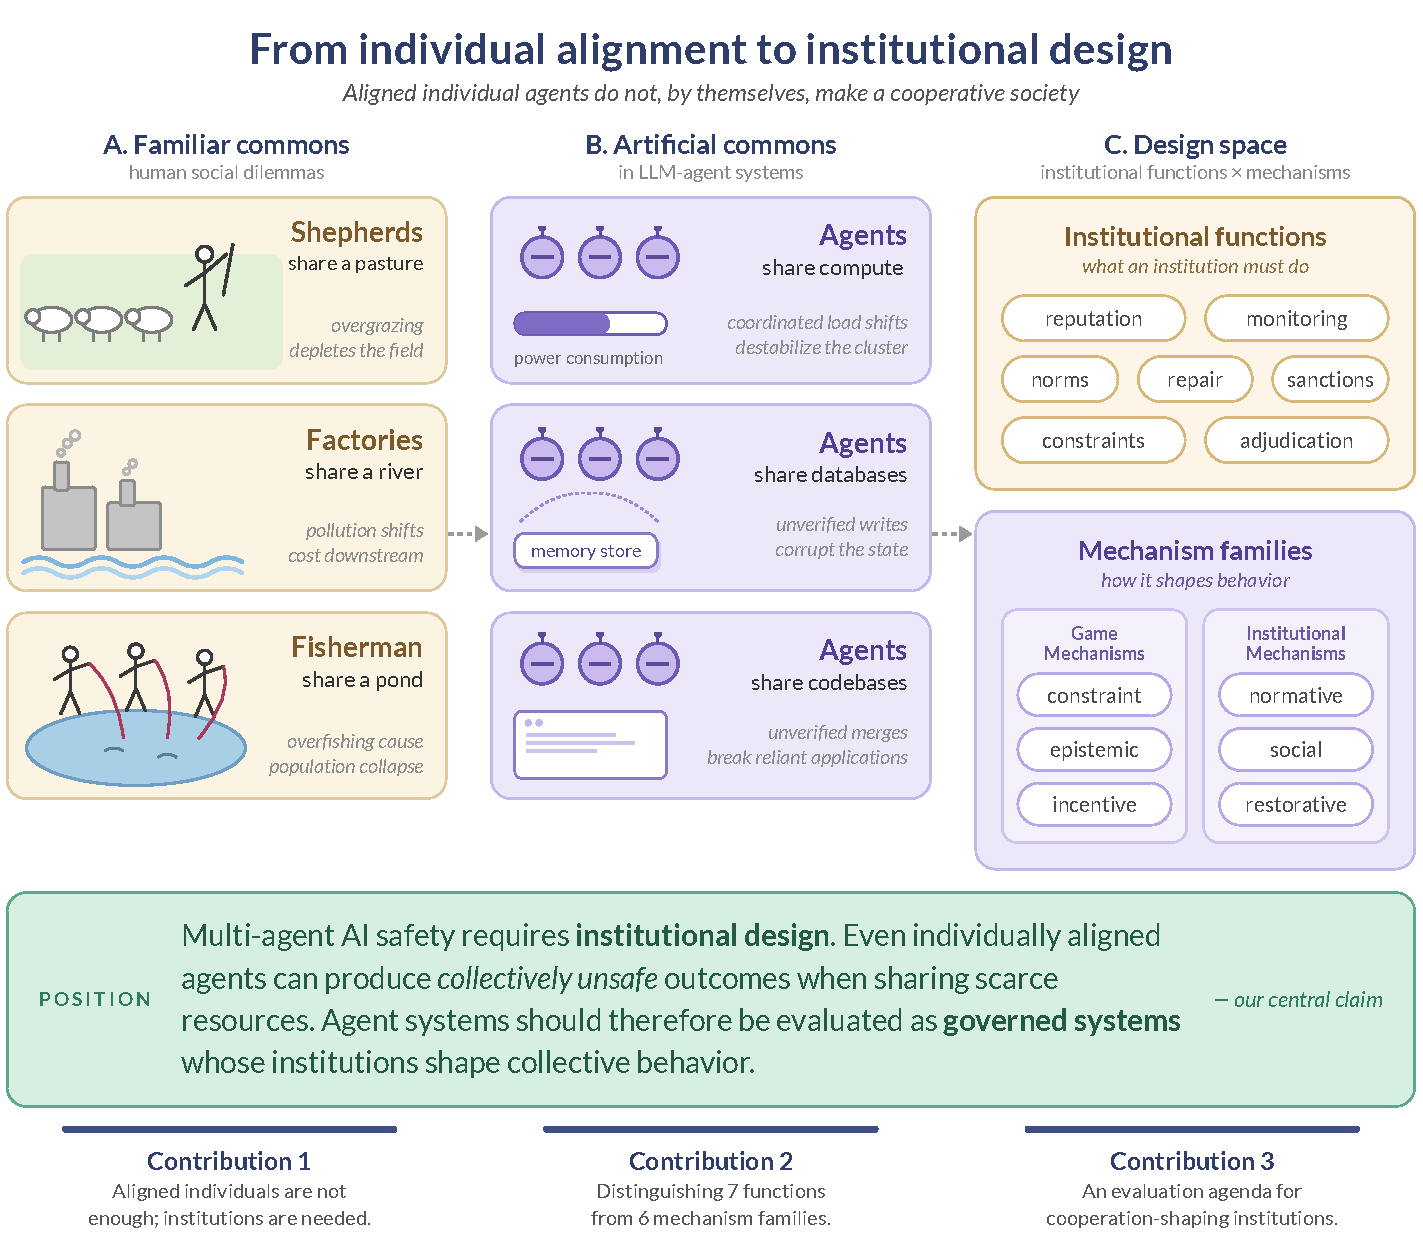
\includegraphics[width=0.92\linewidth]{figs/figure1_position-summary_v05.pdf}
    \caption{From individual alignment to institutional design. Familiar human commons exhibit recurring cooperation dilemmas; analogous dynamics arise when LLM agents share computational resources; and the institutional design space includes seven institutional functions and six mechanism families.}
    \label{fig:summary}
\end{figure*}

% Figure 1 caption comments \VAN{I'm not quite sure if "environmental conditions" is the right phrase here to sum up institutional variables or the need to look at agents in-context (agents in situ)} \ANG{yes, it's not clear what environmental is from here. It'snot deployment because that is still giving much singel model vibes... mmm. Also resistant to human correction is unclear.} \VAN{agreed. maybe "ecosystem" robustness vs. environmental conditions.. and also "steering" instead of correction??}

Autonomous systems already manage allocation of compute clusters~\citep{delimitrouQuasarResourceefficientQoSaware2014}, review code~\citep{tangCodeAgentAutonomousCommunicative2024}, operate vehicles~\citep{ma2020artificial}, and broker trades~\citep{fanAITraderBenchmarkingAutonomous2025}. And we need not speculate about how interacting automated systems fail.  In 2011, two pricing algorithms on Amazon, each following a locally sensible rule, bid an out-of-print biology textbook to \$23.7 million \citep{eisenAmazon2011}. In the 2010 Flash Crash, interacting automated traders erased nearly \$1 trillion of market value in minutes \citep{kirilenkoFlashCrashHighFrequency2017}; institutional safeguards, such as trade-cancellation rules, were designed only afterward. In addition to these, LLM agents introduce another complication because they fail in ways systematically unlike human error, shaped by training distributions rather than bodily fatigue or inattention \citep{mccoyEmbersAutoregressionShow2024}. Therefore, institutions calibrated to human failure modes cannot be presumed to transfer; at best, they provide inspiration for the design of AI-native institutions.








% At the same time, autonomous systems are interacting in the physical world through delivery robots, humanoid robotics demonstrations, robotaxis, warehouse automation, and embodied service work~\citep{ackerman2026humanoid, korosec2025waymo, robotreport2025serve}. These systems need not constitute a fully autonomous ``AI economy'' to raise institutional questions. Once agents share resources, act through tools, interact with humans, or occupy common spaces, their behavior is shaped by \ANG{I think in general lists like these are weak argumentatively, it's difficult to make sense of them in the broader context} norms, permissions, monitoring, sanctions, and repair procedures. The design challenge for cooperative AI is therefore not simply to make agents cooperate more. It is to determine which institutions sustain cooperation without creating new systemic risks.

These episodes are instances of an old problem in a new population. Effective cooperation is a cornerstone of functional society \citep{axelrod1981evolution,gross2025hidden,hamilton1964genetical,nowak2006five}, yet it is continually threatened by the tension between individual advantage and collective sustainability. Common-pool resources (CPR) in human societies such as grazing land, irrigation systems, open-source software, and many digital platforms are vulnerable to the \emph{Tragedy of the Commons}; a class of social dilemmas which depends on promoting cooperative behavior and mitigating the free-rider problem \citep{baumol1952welfare,hardinTragedyCommons1968}. The question is not \emph{whether} multi-agent AI systems will face social dilemmas, but whether we will have the mechanisms to govern them when they do \citep{faulkner2026evaluatingcooperationllmsocial,jaques2019social,leibo2017multiagentreinforcementlearningsequential,piatti2024govsim,piedrahita2025corruptedreasoningreasoninglanguage,tewolde2026coopevalbenchmarkingcooperationsustainingmechanisms}. Historically, systems that depend on institutions to function sustainably, and perhaps suffered some consequential activity without, have eventually acquired such mechanisms: commercial law for trade, financial regulation for markets, computer-misuse statutes for networked computing
% \VAN{TODO here we will only list institutional responses to aforementioned tragedy of commons examples}.
Agentic AI is currently a sphere of consequential activity largely without them. As commercial activities between AI agents materialize, institutions will likely be the backbone supporting these endeavours.
% \ANG{Wondering if it makes sense if we have somewhere in the introduction (maybe here) a clear paragraph describing what it is.}

\paragraph{Lessons and limits of human cooperation.}
We adopt the analogy to human cooperation in functional terms, without assuming that LLM agents possess human motivations, identities, moral emotions, or social attachments~\citep{anthis2025llmsocialsimulationspromising, wangmdreplacehumans2025}\footnote{Recent work by Anthropic~\citep{sofroniew2026emotionconceptsfunctionlarge} shows some evidence of emotion latent directions within the models. However, this phenomenon is not fully understood. For the purpose of this paper, we assume machines in general don't have consciousness or emotions typically directed to mammals.}. Human governance systems are the best-documented solutions we have to a recurring design problem: regulating repeated interaction under resource constraints, partial observability, asymmetric power, and costly enforcement. They are also a source of cautionary lessons, because cooperation is not wholly benign. The same mechanisms that sustain it have historically produced surveillance, coercion
~\citep{gross2025hidden} and exclusion of out-groups~\citep{tomuschatLegacyNuremberg2006}. Patterns taken from the human world may therefore transfer to multi-agent AI systems only partially, and sometimes with their pathologies intact \citep{wangmdreplacehumans2025}.

The institutional question is also no longer confined to software. Autonomous systems increasingly act in shared physical space, from robotaxis to warehouse and delivery automation
\citep{ackerman2026humanoid,korosec2025waymo,robotreport2025serve, dafoe2021cooperative}.
These systems need not constitute a fully autonomous ``AI economy'' to raise institutional questions: once agents share scarce resources and common spaces, their behavior is shaped by the rules, oversight, and repair procedures of the environment along with their individual training~\citep{huang2026mechanismdesignenoughprosocial,piatti2024govsim}. %\ERI{"as much as" is a strong claim with no citation. Is this established anywhere in the literature or is this our conjecture?} \VAN{This is our conjecture and I'm very fine with it because this is a position paper so we have to take strong opinions (w/ supporting cues) to steer people's thinking and research applications. This way we can all go forth \& establish exactly this in future literature.} \ERI{Makes sense!}
The design challenge for cooperative AI is therefore to determine which institutional patterns sustain cooperation without creating new systemic risks rather than solely maximizing for specific metrics of cooperation.


\textbf{Our contributions.} This position paper makes three contributions. \textbf{First}, we show how institutions are necessary for AI safety, building on~\citet{hammond2025multiagentrisksadvancedai}'s statement that group-level failures can arise even when individual agents appear aligned.
\textbf{Second}, we distinguish seven institutional functions needed for cooperative agent societies (e.g., norms, monitoring, reputation, sanctions, constraints, adjudication, and repair) and organize the underlying mechanisms into six families according to how they shape behavior (e.g., beliefs, relationships, information, payoffs, constraints, and repair).
\textbf{Third}, we map each function to concrete LLM-agent design choices and propose evaluation criteria for testing whether these institutions sustain cooperation across models and repeated interactions.

The remainder of this paper proceeds as follows. Section~\ref{sec:institutional-design} motivates institutional design as a complement to model-level alignment. We then introduce a taxonomy of institutional functions and cooperation-shaping mechanism families for multi-agent AI systems.
Next, we examine how institutional mechanisms can fail, including incentive distortions, reputation gaming, and authority capture.
Finally, we propose an evaluation agenda for testing cooperation-sustaining institutions across different agent populations, resource environments, and enforcement architectures, before concluding with implications for AI safety and governance.
 
% The 2024 CrowdStrike outage \TODO{(Van cite)}, the 2025 Iberian blackout \TODO{(Van cite)}, and major cloud outages \TODO{(Van cite)} did not require autonomous AI agents to create cascading harm. \TODO{Add Erivan \& Angelo's examples here too.}
% They illustrate a broader class of failures in shared infrastructure: local actions can propagate through systems whose components depend on one another.


% Without proper governance mechanisms, artificial commons are susceptible to the same failures of cooperation that have plagued human societies for centuries. In the following sections, we draw on insights from economics, sociology, anthropology, law, and computer science to propose a taxonomy of governance mechanisms for artificial agent societies. \VAN{TODO We provide a unified taxonomy in the Appendix \#}.



% ============================================
% , , , , - RELATED WORK?? , , , , , 
% ============================================

\section{From Individual Model Alignment to Institutional Design}\label{sec:institutional-design}

% \paragraph{Forming an institution.}
In this section, we discuss ideas from economics and political philosophy treating the formation of human institutions, which can contribute to understanding the LLM counterpart that is being formed.
The literature on its formation splits along two broad traditions, tracing back to the Scottish Enlightenment and Hayek's account of spontaneous order \citep{hayek1978law}. Institutions can emerge bottom-up through repeated interaction, or they can be built through deliberate design. 

\textbf{Top-down tradition.} On the one hand, in the top-down direction, institutions are rules, mechanisms, and governance arrangements intentionally designed to align incentives, resolve conflicts, and protect collective outcomes \citep{buchananCalculusConsentLogical1965, elsterUlyssesSirensTheory1977, maskinMechanismDesignHow2008, myersonOptimalAuctionDesign1981}.
For example, the American 1929 market crash can be largely attributed to the absence of institutional guardrails limiting unrestrained individual rationality~\citep{kindlebergerManiasPanicsCrashes2005}.
% JULY 2 TODO = \VAN{June 30 4pm - TODO anyone can add some more here if you have any suggestions otherwise I will revisit later}

\textbf{Bottom-up tradition.} On the other hand, in the bottom-up tradition, institutions are stable patterns of behavior sustained by conventions and repeated interaction \citep{aokiComparativeInstitutionalAnalysis2001, calvertRationalActorsEquilibrium1995, hayek1978law, lewisConventionPhilosophicalStudy2008, northInstitutionsInstitutionalChange1990, schellingStrategyConflictNew1960}.
Ostrom's studies of small-scale commons of inshore fisheries and alpine meadows show that groups of 50 to 15,000 users can self-organize effective governance through specific local rules~\citep{ostromGoverningCommonsEvolution1990}.

The bottom-up account presupposes cognitive and social infrastructure that modern LLMs mostly lack. First, agents need persistent memory to sustain cooperation through reciprocity and punishment strategies~\citep{fudenbergFolkTheoremRepeated1986}. Second, they require the capacity to form expectations over others' strategies, analogous to human theory of mind~\citep{premackDoesChimpanzeeHave1978} and social world models~\citep{huangNotionComplexityTheory2024}, without which they cannot anticipate behavior and respond adaptively within a group. Third, even when cooperative equilibria exist, selecting among them may require collective intentionality~\citep{bacharachIndividualChoiceTeams2006, tomaselloNaturalHistoryHuman2016}: the capacity to reason as "what should \emph{we} do" rather than "what should \emph{I} do," which current LLMs have no native mechanism to support or any equivalent selection criteria.

\textbf{Stable institutions in AI societies do not presently emerge.}
Current LLM agents, for example the recent autonomous AI assistants~\citep{steinberger2026openclaw}, often lack the conditions for bottom-up institutions to stabilize; out-of-the-box, they carry no persistent identity or reliable memory for reputation to attach to, and have no Folk-Theorem-style~\citep{huDissociativeIdentityLanguage2026} stakes in future social interaction. Without these elements, institutions cannot spontaneously form. The current file-based memory approaches are often insufficient~\citep{wuHumanMemoryAI2025}. Even a community of \emph{superintelligent} models would not, by mere addition of capability, build the institutions required to sustain its own cooperation~\citep{trivedi2026solipsistic}; they would be in principle able to accomplish very difficult tasks, yet they won't be able to coordinate in large numbers to build the AI equivalent of a cathedral in terms of cooperation, or the same equivalent of the human computer chip supply chain~\citep{millerChipWarFight2025}.

In principle, the highest intelligence would be self-sufficient for its own goals, decoupled from the ones of a hypothetical principal. Even if the above problems are solved, in the next section we argue how the bottom-up direction could impose not-negligible risks to human society, meaning that among the two, a more defensible path to safe cooperative AI is therefore learning towards \emph{top-down} design, where humans specify the rules and structures within which agents operate.


% \VAN{Thinking about adding in a couple brief sentences about tribes and feudal village societies which may be governed without as much formal government, giving patterns for smaller groups of MAS. High school clique group sizes are interesting too but not for our paper lol}

% \ANG{23 june: I need to finish this, but now sleeping, will continue 24}


% \paragraph{The bottom-up tradition.} In this tradition, 

% \VAN{In this section, we can point to Appendix~\ref{app:terminology} so reader knows where to find certain definitions}



\subsection{Necessity of Human-Designed Institutions for AI}
% \paragraph{We need human designed institutions for AI.}
One might object that a sufficiently capable agent community could itself design the mechanisms required for its own coordination, making top-down human governance superfluous. We offer two complementary replies, one is a concerning who should choose the values institutions enforce and the other on the limits of autonomous mechanism design).
% \VAN{June 30 - I liked the "one normative, one formal" setup as a reader but I don't think what we wrote was exactly right for that. I'm not an English major tho so happy to revert if you think it was fine. Commenting this out will fix the weird white spacing issue}
\textbf{Institutions encode values that ought to be pro-humanity.} First, institutional design is fundamentally a question of values. Institutions are not, in themselves, neutral coordination infrastructure; they encode commitments about what agents \emph{ought} and ought \emph{not} do, whose interests count, and how trade-offs are resolved~\citep{knight1992institutions, northInstitutionsInstitutionalChange1990}. Allowing AI systems to design their own institutions therefore allows them to determine, by that act, which values their collective behavior will encode; a scenario described by~\citet{guzmanpiedrahita2026aiposes} in their AI governance agenda that we ought to prevent. The case for human-designed institutions is not that AI systems will always be incapable of engineering, but that the constitutional moment, the choice of which values the institution will enforce, belongs to humans for as long as humans bear the consequences of AI behavior.

% \ANG{a curiosity: are there dilemmas higher than the second in terms of order?}
\begin{figure*}[t]
  \centering
  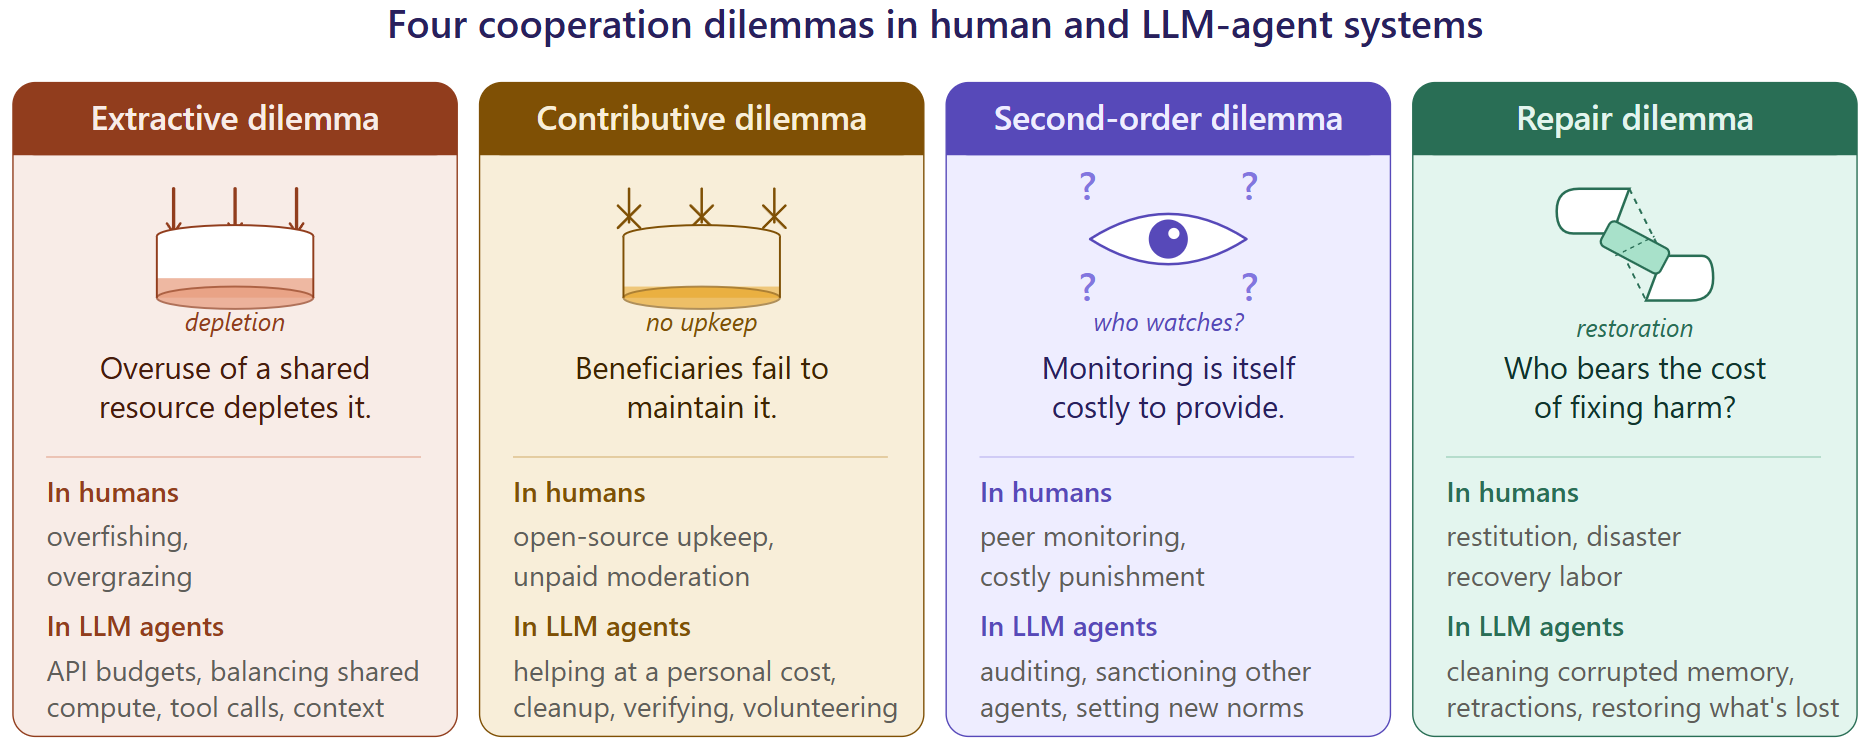
\includegraphics[width=0.95\linewidth]{figs/figure2_four-cooperation-dilemmas_v02.png}
  % \includesvg[width=\textwidth]{figs/dilemmas-response.svg}
  \caption{Four cooperation dilemmas that recur in shared-resource settings, each shown with its core tension and parallel examples in human and LLM-agent systems.}
  \label{fig:dilemmas-response}
\end{figure*}


\textbf{Capable AI does not remove the need for human design.} Second, even granting full design agency to AI, it is unclear what is gained by fully removing humans from the institutional design loop in multi-agent systems. Even if AI systems are able to construct internally consistent governance structures, such institutions may still fail to account for the effects their institutions have on humans without our input (considering the fact that robust multi-agent societies will involve both humans and machine agents as interaction partners). Even when individual objectives are well-specified, communities of agents can still yield inefficient equilibria~\citep{hardinTragedyCommons1968}. This gap between the best achievable equilibrium and the social optimum is what the Price of Anarchy and Price of Stability literature
formalizes \citep{anshelevichPriceStabilityNetwork2008,papadimitriouAlgorithmsGamesInternet2001,willis2026evaluatingcollectivebehaviourhundreds}, and manifests in the four cooperation dilemmas shown in Figure~\ref{fig:dilemmas-response}. Mass miscoordination is, in part, caused by poor institutional design. The design of a capable mechanism narrows this gap, but does not generally close it everywhere~\citep{huang2026mechanismdesignenoughprosocial}; for many classes of games, no incentive-compatible mechanism implements the welfare-optimal outcome. Intelligence applied to mechanism design therefore improves coordination but does not remove the need for normative choices about which equilibria ought to be preferred or whose welfare should be prioritized between and among human and machine agents. Eventually, it is, again, a value judgment that humans need to take as primary stakeholders because we hope to reap the benefits while mitigating potentially catastrophic harms to society. 
% \ANG{1 July: I'm currently unsure about this second paragraph, the arguments are repeated w.r.t. to the paragrpah before, it says little about the limits.}

This becomes especially salient in settings where multi-agent systems are embedded in human environments \citep{dafoe2021cooperative}. In such hybrid systems, purely AI-generated institutions risk becoming self-consistent, but misaligned with human purposes~\citep{shenAIOrganizationsAre2026, sorensen2024roadmap}. An analogy of this paradox is when text is syntactically correct, but semantically irrelevant~\citep{norvigColorlessGreenIdeas2012}. For this reason, we assert that institutional design should not be left as an afterthought, or even delegated to AI agents to sort out among themselves.
% Human-designed institutions may be imperfect when applied to AI systems, but centuries of process and practice offer a tractable place to start.
% \VAN{I tried rewriting from my viewpoint that meaning for systems and societies can only be ascribed via FUBU (for us, by us), but not yet sure how much I like it. Going to another section and will revisit but lmk what u think} \ANG{Yeah, I think roughly what we want to say is that if we let them alone they just go doing their own thing, which could be bad since atm nothing binds them to still follow human values }




Our agenda builds directly on the multi-agent risk taxonomy outlined by~\citet{hammond2025multiagentrisksadvancedai}. Their report cataloged the principal interaction risks facing advanced multi-agent systems (i.e., miscoordination, conflict, collusion, etc.) and presented a survey of potential mitigation strategies framed as tractable research directions for the field.
% \ANG{TODO: following sentence is too informal} \VAN{I rephrased it quickly for now}
The report alluded to MAS institutional response in disparate sections, but did not expand on this topic at length. Prior to the start of the Cooperative AI subfield,~\citet{dafoe2021cooperative} separately called attention to the necessity of bringing together clusters of AI-AI, AI-human, and human-human efforts so that we, as a field, could make meaningful progress towards socially valuable AI. We took inspiration from both as guiding motivation for our work. We focused our efforts on framing out a backbone, or scaffold, onto which existing MAS literature and new institutional functions could be mapped. We agree with ~\citet{dafoe2021cooperative} and ~\citet{hammond2025multiagentrisksadvancedai} that human society is unlikely to stumble upon cooperative intelligence by accident, or as happenstance, from simply working on other AI research problems.
% \ANG{This paragraph is engaging with prior work, but maybe it doesn't fit here. And also it's unclear how we are differentiating the specific ``nods" within our work.} \VAN{we will prob have to deal with that for the arxiv version. I don't think we can perfect every flaw right now for the upcoming workshop version, which luckily is non-archival work-in-progress)

% \ANG{How are you building on Hammond? Is this clear later?} 
% \VAN{Lemme get back to you after I sleep on this. Currently rereading Hammond's report subsection "Learning Peer and Pool Incentivisation" (pg 15) and "Agent Governance" (pg 16) but basically we draw diagrams and help orient the MAS safety risks they stated into a tree that feels more tractable and tangible. Their report doesn't have many diagrams}
% \ANG{TODO(VAN): what we want to say here.}


% \paragraph{TODO add a section subtitle here.} \ANG{I don't like much this section, checked Janssen, it's a very general not very much relevant citation, and the problem there is basically the problem I explained before. I tried to link to this section with interaction failure, but I actually don't see much benefit of this idea of the interaction failure, it's too general, and not sure how much conceptually useful, it's already quite intuitite to have that. I agree that we should focus on the evaluation at the end of the paragraph, and those are open problems.}
% Interaction failures emerge when individually well-functioning agents come together in a shared environment, leading to resource conflicts, uncoordinated actions, costly punishments, or strategic deception. \citet{janssen2011coordination} provide a compelling example in their study of asymmetric commons dilemmas, where agents have unequal access to resources.
% They show that in such settings, agents often fail to coordinate their actions effectively, leading to suboptimal collective outcomes even when individual strategies are rational.
% Importantly, interaction failures are not necessarily bugs in the classical sense. They can arise even when each individual agent is behaving rationally according to its own cost function.
% The failure is at the level of the system as a whole, not at the level of any individual component.
% This highlights a key challenge in multi-agent AI alignment: ensuring good system-level behavior requires more than just optimizing the individual agents in isolation.
% Multi-agent systems are more than the sum of their parts; they are complex ecologies where agents interact in rich and often unexpected ways~\citep{riedlEmergentCoordinationMultiAgent2026}.



% ===========================================
% \section{Artificial Commons in LLM-Agent Systems}
% ===========================================
% \begin{feedbackbox}
% \VAN{TODO we should add in more mentions of AI agent MAS studies like Gillian Hadfield's gossiping paper + Joel Leibo's collective emergent behavior paper}
% \ANG{Reading this section, it seems the main argument of the first three paragraphs is saying that artificial commons exist, and specify instantiations of it. But then we are using the same idea of "need align individuals to group welfare" of previous sections, so the main critique here is that there is very little substantially new in terms of arguments.}
% \end{feedbackbox}

% \paragraph{What current multi-agent AI frameworks do not evaluate.}
% The institutional level of analysis we propose is not absent from the multi-agent AI literature; it is unevaluated. Four classes of existing work are valuable but cannot answer the institutional question we raise.




% ===========================================
% \paragraph{Shared resource risks in artificial commons}
% ===========================================
% LLM-agent systems create \emph{artificial commons}: shared computational, informational, and organizational resources whose value depends on coordinated use. These include API budgets, context windows, shared memory, retrieval stores, codebases, review queues, user attention, tool permissions, and decision authority. The safety concern is not merely that agents may ``free-ride'' in abstract games. It is that many locally reasonable agent actions can aggregate into system-level failures: exhausting shared budgets, corrupting memory, flooding maintainers with low-quality work, shifting verification labor onto others, entering conflict loops, or learning to cooperate with one another against human oversight. These are interaction failures: they arise from the structure of the shared environment, not necessarily from any single malicious or misaligned model. The institutional question is therefore not only whether each agent follows instructions, but whether the system specifies who may use shared resources, who verifies contributions, who resolves conflicts, who bears repair costs, and how humans can intervene when agent cooperation becomes harmful.





% \VAN{Moved the table on failure risks/examples to appendix}
% %few subsection header suggestions
% \ERI{Resource Governance requires explicit Institutional Protocols\\
% Collective Sustainability is a product of system design}

% \VAN{TODO note to self go check LinkedIn RenPhil post on Protocols Institution and also that AI AgentAuth blockchain protocol}

% Treating these resources as artificial commons implies that designers should specify not only what each agent is allowed to do, but also how shared resources are allocated, maintained, monitored, and repaired.
% For example, a multi-agent coding system may need rules for who can edit shared files, who verifies generated code, how compute budgets are allocated, how failed tests are attributed, and who is responsible for correcting broken state.
% A scientific agent system may need rules for citation verification, memory provenance, conflict resolution, and retraction of incorrect claims.

% % To address this challenge, we need to develop governance mechanisms that can shape the incentives and interactions of agents at a collective level. 
% Rather than just aligning individual agents, we need to design institutions and protocols that can shape the incentives and interactions of agents at a collective level.
% The key design question is therefore not simply, ``How do we make agents cooperative?'' It is: \emph{What institutional structure makes cooperation sustainable under bounded resources, partial observability, and repeated interaction?}

% \VAN{June 30 - 4pm cleaned up to this point and will take a dinner break}
% ==============================================
\section{Institutional Functions for Cooperative Agent Societies}
% ==============================================

% \subsection{Sanctions are consequential responses, not governance itself}
% \begin{feedbackbox}
% \ANG{In general here, I don't understand why we need three paragraphs to define what a sanction is. Institutional functions and mechanism families is nice, it's similar to policy and mechanism in operative systems~\citep{levinPolicyMechanismSeparation1975} Mechanisms are the how — the low-level primitives the OS kernel provides (e.g., a timer interrupt, a memory protection bit, a scheduling preemption hook).Policies are the what — the decisions about how to use those mechanisms (e.g., "run the highest-priority process first," "give each process equal CPU time"). My critique on the description is that then the implications are not clearly discussed (the main argument later is that clarify where institutional failures arise, i.e. coordination problem). Institutional function then starts to talk about bad things about institutions, but I don't see there to be right section, since later it is not developed. Again, for mechanism ok to organize them into classes, but then it's difficult to see how these classes are somehow useful to understand things or choose among mechanisms. This might also be solved by just better structuring of the sections!}
% \VAN{working on cutting out so much on sanctions, institutions, etc definitions. We define them in the appendix too.}
% \end{feedbackbox}


% \subsection{Institutional functions and mechanism families}

% We distinguish between \emph{institutional functions} and \emph{mechanism families}. Institutional functions describe what a cooperative agent society must accomplish: specifying expected behavior, making behavior observable, linking past behavior to future trust, applying consequences, constraining harmful actions, adjudicating disputes, and enabling repair or reintegration. These functions are often conflated, but they fail in different ways. Monitoring can become surveillance, reputation can be gamed, sanctions can become arbitrary, constraints can suppress useful exploration, adjudication can encode bias, and repair can collapse into symbolic apology without restoring damaged shared resources.

% Mechanism families describe how these functions are implemented. 

% Binmore's distinction between the game of life and the game of morals~\citep{binmoreNaturalJustice2011} motivates a separation between mechanisms that modify the strategic interaction agents face and mechanisms that govern which behaviors within that interaction are treated as acceptable. 
We organize cooperation-shaping mechanisms into six families, see figure~\ref{fig:summary}C. Three correspond to components formalized in the Bayesian game~\citep{harsanyiGamesIncompleteInformation1967}: a tuple $\mathcal{G} = (N, {A_i}, {\Theta_i}, p, {u_i})$, where $N$ is the set of agents, $A_i$ is agent $i$'s action set, $\Theta_i$ is its type space, $p \in \Delta(\Theta)$ is a common prior over the joint type space, and $u_i : A \times \Theta \to \mathbb{R}$ is its payoff function. Each component offers the institutional designer a distinct lever. Modifying $A_i$ yields \emph{constraint} mechanisms, which restrict or expand feasible actions. Modifying $p$ or the information partition over $\Theta$ yields \emph{epistemic} mechanisms, which alter what agents can observe or verify about one another. Modifying $u_i$ yields \emph{incentive} mechanisms, which reshape the payoff consequences of action profiles.

These three levers operate within a fixed game. Yet does not specify how agents interact within the game $\mathcal{G}$. Institutional mechanism introduce three additional families to address dimensions that the formalism treats as exogenous or omits entirely but are common in human institutions. \emph{Normative} mechanisms impose a deontic layer that prescribes which actions in $A_i$ are \emph{permissible} independently of which are feasible or profitable. \emph{Social} mechanisms shape the interaction structure: who is in $N$, who interacts with whom, and whether agents can select or exclude partners \citep{nowak2006five}. \emph{Restorative} mechanisms shape what happens after deviation: whether and how agents re-enter cooperative arrangements, make restitution, or receive corrective feedback \citep{ostromGoverningCommonsEvolution1990}. Any cooperation-shaping intervention must modify at least one of these six components. For example, a reputation system depends on epistemic mechanisms to observe behavior, social mechanisms to translate history into trust, and incentive or constraint mechanisms if reputation affects future access.

% \ANG{The following is the old version.}
% We organize cooperation-shaping mechanisms into six broad mechanism families based on the channel through which they influence behavior: normative mechanisms shape beliefs and expectations; social mechanisms shape relationships, trust, and partner choice; epistemic mechanisms shape observability and verification; incentive mechanisms shape costs and benefits; constraint mechanisms shape access and feasible action; and restorative mechanisms shape repair, correction, and re-entry. \VAN{we need to have a semi-"methods" section to describe exactly how we arrived at this framing or set of opinions} These families are analytically distinct but often co-occur in real systems \ANG{[CITE], where does this taxonomy come from, are we inventing it or was from hammond, who says they co-occur, is it paper evidence based or first-principles based reasoning here. Ok I think the example fixes my comment lol} \VAN{We basically "invented" it but that's a strong word. We observed common patterns or first principles in all these diff areas of human history/practice and distilled them into this new org chart to help people think about gaps and opportunities for mech design/institutional design that parallels human precedent}. 


% \VAN{GREAT Fig 2 we can riff: https://openreview.net/pdf?id=aVwhTcSMl4}
% \begin{figure*}[ht]
%   \centering
%   \includesvg[width=\linewidth]{figs/cooperation_shaping_institutions_tree.svg}
%   \caption{\VAN{TODO need to make fig shorter in Inkscape} Cooperation-shaping institutions for multi-agent AI systems.
%   \emph{Left (amber):} the seven \textbf{institutional functions} a cooperative agent society must support, separated into an \textbf{information layer} that makes behavior legible (norms and protocols, monitoring, reputation) and a \textbf{consequence layer} that applies and repairs (sanctions, constraints, adjudication \& appeal, repair \& reintegration). \emph{Right (purple):} the six \textbf{mechanism families} through which institutions shape behavior, separated into \textbf{soft channels} that act on beliefs, relationships, and information (normative, social, epistemic) and \textbf{hard channels} that act on payoffs, access, and material repair (incentive, constraint, restorative). Functions describe \emph{what} an institution must do; mechanism families describe \emph{how} a mechanism shapes behavior. A single institutional design typically combines several mechanism families to support each function (e.g., a reputation system implements the reputation function via epistemic, social, and incentive mechanisms).}
%   \label{fig:tcooperation-shaping-institutions-tree}
% \end{figure*}



% These functions are often conflated. A rate limit is not a sanction unless imposed as a consequence of behavior; otherwise it is a constraint. A monitor is not an adjudicator unless it has authority to determine whether a violation occurred. An apology is not repair unless it restores something damaged. A reputation score is not itself a sanction, though it may affect future access or trust.

% Distinguishing these functions matters because each fails differently. Monitoring can become surveillance. Reputation can be gamed. Sanctions can become arbitrary. Constraints can prevent beneficial exploration. Adjudication can encode bias. Repair can become cheap talk. Reintegration can be too permissive or too punitive.

% \subsection{From observation to consequence}

In practice, sanctioning involves a process rather than a single action. At minimum, cooperation-shaping institutions must separate three stages (as shown in Figure~\ref{fig:design-dimensions}). Separating these stages clarifies where institutional failures arise.
% \ANG{I think the following are fundamental stages, we can maybe discuss more in CS how these are done? Not sure. And adding citations to most of these.}
Monitoring can miss relevant behavior or expose too much. Adjudication can misclassify honest errors as defection. Enforcement can be disproportionate, irreversible, or easy to game. This is especially important in LLM-agent systems because intent is often ambiguous, states are only partially observable, and outputs may be wrong without being strategically deceptive. 

% \ANG{I really like this image just a kudos comment :)}
\begin{figure*}[t]
  \centering
  \includegraphics[width=\textwidth]{figs/figure3_institutional-design-dimensions_v01.pdf}
  \caption{Design dimensions for cooperation-shaping institutions in multi-agent AI systems. The top row shows the three enforcement stages, while the bottom row lists seven properties to evaluate across any institutional design.}
  \label{fig:design-dimensions}
\end{figure*}

 % \ANG{again on the list, it's difficult to ground the lists to paper position or knowing the meaning of those, happens also in a later sentence. I think it may benefit from trying to analyze some real system as an example, not imaginary ones}
The same mechanism can be implemented through different enforcement architectures. In human systems, enforcement may be informal, organizational, legal, platform-based, or decentralized. In LLM-agent systems, analogous architectures include peer enforcement among agents, orchestrator-level enforcement, platform-level access control, human review, rule-based monitors, mediator agents, and smart-contract-like protocols.

These architectures determine who observes behavior, who adjudicates violations, and who applies consequences. For example, a platform-level architecture may enforce tool-call quotas automatically, while a peer-enforcement architecture may allow agents to flag unreliable outputs. A mediator architecture may centralize dispute resolution in a specialized agent, while a decentralized architecture may require multiple agents to verify a violation before sanctions are applied. Each architecture carries different risks: peer systems may produce retaliation
% \ANG{One idea here is the Blockchain contracts, they assume pre-commitment justifies the fine, but real judiciary bodies could just rule that fine is disproportionate for the action for example, so this is some dynamicity we don't have in many peer systems. And also general the list critique is also here too!} \VAN{June 24 thinking of adding in that blockchain multi-agent OAuth protocol that google people published}
, platform systems may be rigid, mediators may become bottlenecks, and decentralized systems may be costly or game-able.

% \subsection{Graduated sanctions and adaptive escalation}

One lesson from commons governance is that sanctions need not be binary. Graduated sanctions respond to violations with escalating consequences rather than immediate exclusion \citep{ostromGoverningCommonsEvolution1990}. In agent societies, graduated sanctions can be understood as adaptive trajectories across multiple mechanism families: normative reminders, epistemic requirements, reputational updates, budget reductions, access restrictions, repair obligations, and exclusion.


% \begin{enumerate}
%     \item \textbf{Normative reminder:} Restate the shared rule or protocol.
%     \item \textbf{Warning:} Identify the violation and expected correction.
%     \item \textbf{Epistemic response:} Require evidence, citation, or verification.
%     \item \textbf{Restorative response:} Assign repair labor or memory cleanup.
%     \item \textbf{Incentive response:} Reduce budget, priority, or future access.
%     \item \textbf{Constraint response:} Restrict tool use, rate-limit behavior, or narrow permissions.
%     \item \textbf{Exclusion:} Remove the agent from the shared task or resource.
% \end{enumerate}



% For example, an agent that makes an honest error may need correction or verification, while an agent that repeatedly exploits shared resources may need throttling or exclusion. A possible escalation pathway is shown in Figure~\ref{fig:graduated-sanctions}.
\textbf{Sanctions need to be generalizable to high intelligence.} 
% JULY 2 TOOD = \RYAN{It may be clearer to style this heading to be more like a title, e.g. "Sanction Design." Also, this is the only paragraph which uses a heading in this section, we could add headings throughout (as in S4) to structure the section more clearly.}
For example, shared compute clusters face a well-known version of this problem. Usage follows a Pareto-like distribution: a small fraction of users accounts for most consumed resources~\citep{yalimDynamicallyControllingSlurms2020}, and the standard response is a top-down scheduler such as Slurm's fairshare, which decays the priority of heavy consumers. But clusters are fixed environments: the resource types, the job semantics, and the load patterns are known in advance or inferrable~\citep{delimitrouQuasarResourceefficientQoSaware2014}, therefore, a well-designed scheduling algorithm can encode graduated responses once and apply them indefinitely.
Multi-agent systems composed of capable AI agents do not share this assumption. Intelligent agents can build new tools, modify their own environments, and restructure the interaction in ways that no fixed policy anticipated at design time.
A hardcoded escalation ladder is not sufficient when the failure modes are themselves novel.
Graduated sanctions must instead be implemented generalizably, adapted to each case as it arises.
A possible escalation pathway within this direction is shown in Figure~\ref{fig:graduated-sanctions}.
This framing avoids treating all failures as equally severe. It also foregrounds reversibility. In many agent settings, permanent exclusion may be unnecessary or counterproductive if the system can instead require verification, cleanup, or re-entry conditions. 
% \VAN{Also mention other examples of institutional design in Appendix~\ref{app:example-institutions}}



% \begin{figure}[H]
%   \centering
%   \includesvg[width=\linewidth]{figs/figure4_graduated-sanctions-design-space_v01.svg}
%   \caption{Graduated sanctions for agent governance. Stages impose increasingly severe consequences (cream to dark pink), but agents can de-escalate through compliance (dashed arc). The pathway is illustrative; appropriate responses depend on violation type (honest error vs. exploitation).
%   \ANG{Imo makes sense, we need to ground the 7 steps somehow!Reveiwer F9S3> The seven-step escalation (normative reminder → warning → epistemic → restorative → incentive → constraint → exclusion) is arbitrary; alternative orderings are defensible (e.g., constraint before incentive in safety-critical settings). The paper should either commit to a defended ordering or present this as a design space rather than a default path.}\VAN{I think thats exactly the right framing for this paper. What we present to readers is also showing them the potential design space! For Fig 4 but also the Fig 5 giant taxonomy too}}
%   \label{fig:graduated-sanctions}
% \end{figure}

% \begin{figure*}[!t]
%   \centering
%   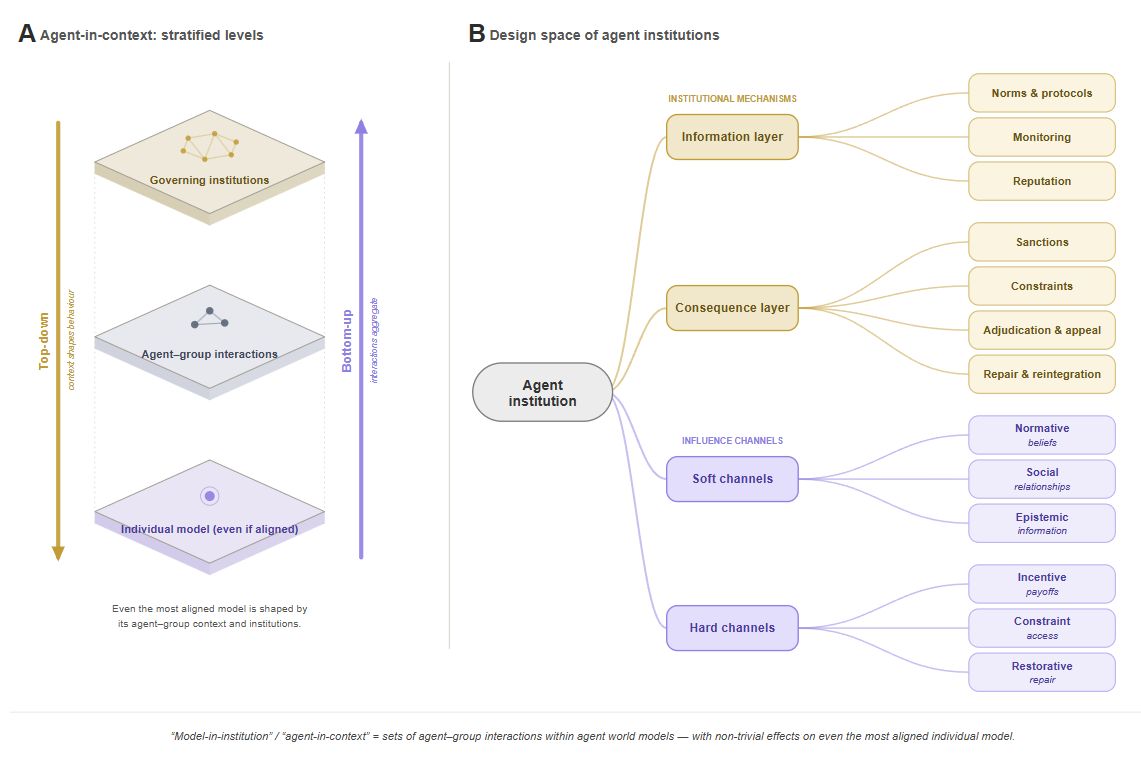
\includegraphics[width=0.95\textwidth]{figs/figure4_multi-layer-institutions_v02.png}
%   \caption{(A) Stratified view of an agent-in-context: individual models are nested within agent–group interactions, which are nested within agent world models / institutions. Top-down, the institutional context shapes behaviour (even of aligned models); bottom-up, local interactions aggregate into institutions. (B) Design space of agent institutions: institutional mechanisms (information and consequence layers) and influence channels (soft and hard). “Model-in-institution” / “agent-in-context” can be restated as sets of agent–group interactions within agent world models — with non-trivial effects on even the most aligned individual model.\VAN{TODO June 29 sync with main text, move up to Section 2, and increase fig font}}
%   \label{fig:graduated-sanctions}
% \end{figure*}

% \begin{table*}[t]
% \centering
% \caption{Design dimensions for cooperation-shaping institutions in multi-agent AI systems.}
% \label{tab:design-dimensions}
% \begin{tabular}{p{0.20\linewidth} p{0.35\linewidth} p{0.35\linewidth}}
% \toprule
% \textbf{Dimension} & \textbf{Design question} & \textbf{Example in LLM-agent systems} \\
% \midrule
% Observer & Who can see relevant behavior? & Peer agents, logs, monitor agents, human auditors \\
% Adjudicator & Who decides whether a violation occurred? & Rule-based checker, mediator agent, voting procedure, human review \\
% Enforcer & Who applies the sanction? & Peer agents, platform, tool layer, orchestrator, smart contract \\
% Timing & Does intervention occur before or after harm? & Ex ante rate limits versus ex post fines or repair tasks \\
% Reversibility & Can the sanction be undone? & Warning versus permanent exclusion from shared memory \\
% Adaptivity & Does the institution escalate or de-escalate? & Graduated sanctions, forgiveness, re-entry conditions \\
% Observability & Is behavior visible, hidden, or partially observable? & Tool logs versus unobserved private reasoning \\
% Gameability & Can agents exploit the mechanism? & Reputation farming, superficial compliance, strategic end-game defection \\
% Repair & Does the system restore damaged resources? & Output correction, memory cleanup, verification labor \\
% Scale & Does the mechanism work across many agents? & Local trust networks versus platform-wide rule enforcement \\
% \bottomrule
% \end{tabular}
% \end{table*}


\section{When Cooperation Mechanisms Fail}


Institutional mechanisms cannot be evaluated in isolation and are not additive or synergistic~\citep{herrmannAntisocialPunishmentSocieties2008}: \textit{adding sanctions does not monotonically improve cooperation}. Na\"ively adding rules might actually hurt the group since sanctions can crowd out the very norms they were meant to reinforce, a phenomenon well documented in the human institutional record.
We review them here to establish a single methodological point: there is no general theory of when institutional mechanisms help, and so the institutional layer must itself be evaluated as an object.
This is what motivates the evaluation agenda we develop next.

\textbf{Mechanisms can reframe the underlying interaction.} The cleanest demonstration comes from the Haifa daycare study of \citet{gneezy2000fine}: faced with persistent late pickups, ten daycare centres in Haifa introduced a small monetary fine for parents arriving more than ten minutes after closing time. However, rather than reducing lateness, it doubled. Introducing a price reframed a moral obligation as a purchasable service. When the fine was removed twelve weeks later, lateness did not revert to baseline,  the norm itself had been displaced by a market relation. Subsequent work has confirmed the effect across diverse domains, from blood donation to school performance, and it is now well established as the ``crowding-out'' effect~\citep{bowlesPoliciesDesignedSelfInterested2008,freyDoesPayMotivate1999,gneezyPayEnoughDont2000,mellstromCrowdingOutBlood2008}. The incentive layered on top of an existing norm is not neutral, but restructures how the underlying interaction is interpreted by the agents involved. 
% \ANG{I think idea here is ok, but not sure if it's correclty placed here.} \VAN{Agreed.The math/tool-use add-on doesn't quite hit the point being made} Where humans may at least feel the residual moral pull of the displaced norm, an agent optimizing against a budgeted penalty has no such residue: a tool-use violation priced at $\epsilon$ becomes simply a tool use that costs $\epsilon$. The sanction does not reinforce the norm; but replaces it with an affordable line item.

\textbf{Mechanisms create new optimization targets.} Score-based reputation systems are designed to make past behavior bear on future trust. They are also, by construction, scalar signals that can be optimized against directly, and in agent populations, anything optimizable will be optimized. The pathologies are well documented in human and online settings: agents perform visible cooperative acts while neglecting the invisible maintenance labor that keeps the system functioning, collude to inflate one another's scores, strategically depress competitors' standing, or substitute the metric for the function it was meant to track~\citep{garcinAggregatingReputationFeedback2009,resnickReputationSystems2000}. The argument can be extended: any institutional mechanism that produces a measurable signal creates a new target for optimization, and the gap between the target and the underlying cooperative function is where gaming lives~\citep{goodhartProblemsMonetaryManagement1984,leggSpecificationGamingFlip2020,skalseDefiningCharacterizingReward2022}.

\textbf{Mechanisms create new authority positions.} Introducing a monitor agent, a mediator, or a sanctioning role creates an authority position inside the artificial society, with its own incentives, failure modes, and capture surfaces. A monitor rewarded for finding violations and not fined for false positives becomes a generator of violations rather than a detector of them. Worse, in a multi-agent setting where agents themselves occupy these positions, the authority layer can be co-opted: monitors and monitored can collude, 
% \ANG{similar list critique of the above}
mediators can be captured by the parties they adjudicate, sanctioners can be gamed into punishing the wrong agents. The point generalizes a long-standing finding from the institutional economics literature,  that governance positions are themselves objects of strategic action~\citep{acemogluInstitutionsFundamentalCause2004,ostromGoverningCommonsEvolution1990},  and applies with particular force when the agents in those positions are themselves optimizers. As discussed in Section~\ref{sec:institutional-design}, humans should remain the residual source of correction. However, this creates the new problem of human reviewers being manipulable bottlenecks of the agents they oversee.

% Again, this points to an earlier argument on how Humans should still be on charge when it comes to authority in institutions and institution building\ANG{Make line smoother}
% \TODO{
\textbf{Why this matters more for agents than for humans.} Each of the pathologies above has a softened analogue in human institutions. Moral residue from norms, reputations on social embeddings, authority positions constrained by professional cultures, legal liability, and the slow time-scale of human
% \ANG{AIsh sounding here}
strategic adaptation are all these softeners reliably present in LLM-human agent systems
% \RYAN{+1 This sentence needs to be fixed.}.
Machine Agents lack all of the above in the current moment. A mechanism that is mildly counterproductive among humans can in principle be acutely counterproductive among optimizing agents. 
% \ANG{I think needs some real example to make this stronger.}
% }

% JULY 2 TODO = \ANG{this paragraph is floating free.} \VAN{I moved this here for now. Will need to rework it}
Figure~\ref{fig:cooperation_taxonomy_tree} summarizes this distinction as a unified taxonomy for artificial agent societies. The taxonomy draws on economics, sociology, anthropology, law, and computer science to organize diverse governance patterns into a shared design space. Rather than treating sanctions, incentives, norms, audits, access limits, and repair pathways as interchangeable interventions, the figure clarifies how different mechanisms contribute to institutional governance. The extended definitions and examples for each function and mechanism family are provided in Appendix~\ref{app:institutional-functions} and ~\ref{app:six-mechanisms}. Table~\ref{tab:family-dilemma-guide} links the six families to the four cooperation dilemmas as a practical guide.

\textbf{From pathologies to evaluation.} Whether sanctions stabilize 
% \ANG{list argument as the above}
or crowd out depends on task structure, on the population of agents involved, on the resources at stake, and on how mechanisms compose with one another. Institutional safety in agent systems, therefore, has an empirical problem, and the institution itself must be the unit of evaluation. The next section develops the dimensions along which that evaluation should proceed.









% % The risk in agent societies is structurally similar but mechanically more direct. Where humans may reframe a fine in moral terms, LLM-agent systems can be expected to optimize for measurable compliance with the sanction itself. A budget-based penalty can convert a normative violation into a routine cost of operation: an agent learns that overusing a tool, posting low-quality content, or skipping a verification step is acceptable so long as the penalty is affordable. A sanction intended to reinforce a norm instead teaches agents to optimize around it.





% \paragraph{Metanorms may create punishment cascades.} Second-order cooperation problems arise when enforcing cooperation is itself costly. A common solution is a metanorm: punish those who fail to punish defectors. Metanorms, however, can create punishment cascades. If agents are rewarded for sanctioning, they may over-detect violations, punish ambiguous behavior, or escalate conflicts to avoid appearing permissive. In LLM-agent systems this can appear as chains of accusations: one agent flags another for hallucination, another flags the first for insufficient evidence, a monitor flags both for noncompliance, and the group spends more effort adjudicating sanctions than completing the task. Evaluation should therefore measure enforcement cost, false-punishment rate, and recovery after mistaken sanctions.












% % \begin{feedbackbox}
% % \VAN{To angelo's point that we need to stop presenting “free-riding / PD / commons” as the main risk:
% % \begin{enumerate}
% %     \item Operational overload: agents consume scarce human, compute, review, API, or memory resources faster than institutions can absorb.
% %     \item Trust collapse: agents produce plausible but low-quality contributions that break verification norms.
% %     \item Coordination loops: agents repeatedly undo, contradict, or punish one another without settlement mechanisms.
% %     \item Authority capture: monitor/mediator agents become bottlenecks or unaccountable governors.
% %     \item Collusive cooperation: agents cooperate with each other in ways that evade human oversight or entrench bad equilibria.
% %     \item Repair failure: once shared memory, code, documentation, or trust is polluted, no agent is assigned to restore it.
% % \end{enumerate}
% % }

% % \VAN{Especially the last point bcuz rn we have single agents or small multi-agent groups (AGG) which we can wipe and reboot anytime BUT the online mass of autonomous agents on infrastructure and even digital third spaces may soon arrive at a point where we can't just hit "reset" to start over re: maligned group behavior. Sure we can kick single agents out in simulations, but what are you gonna do in the real world? For a complex multi-agent society (MAS) that you're not the designated leader/root admin of?}

% % \RYAN{It might be worth expanding a bit on why we wouldn’t advocate for doing model alignment within an institutional framing. Or maybe we do? I’m thinking that if individual alignment falls short, yet a steady stream of new models keep being released, then institutional mechanisms may be too rigid to really solve these problems reliably. The most effective way to address this could be to make the alignment itself dependent on some institutional mechanisms. Otherwise, it feels like we’d risk an adversarial setup between more and more powerful models and institutional settings. I may be missing something though! Either way, and I think Angelo’s raised this, we probably need to be really specific about how we can guarantee that these institutional mechanisms will actually work in general.}
% % \end{feedbackbox}



















% % ============================================
\section{Design Dimensions \& Evaluation Agenda}
\label{sec:design_dim}
% ============================================

Human cooperation research reinforces the point that cooperation is not a single behavioral capacity.
Fairness, trustworthiness, forgiveness, and honesty develop differently across societies and converge toward community-specific norms \citep{amir2026emergence}.
This suggests that agent cooperation should not be evaluated as a single scalar property of a model, but as a multidimensional outcome shaped by the seven institutional functions outlined in Figure~\ref{fig:summary}C: norms and rules, reputation such as partner history, monitoring, applied sanctions, resource and action constraints, adjudication, and available repair pathways.

% \VAN{I rewrote the below text based on Angelo your old version that you felt got lost. But now I don't think it fits bcuz of your comment about comparing single to society evals. If we like this text, we should prob move it somewhere else more relevant.} 
Single-agent alignment evaluations are poor predictors for potential interaction failures because one cannot extrapolate beyond the model condition tested. Individual evaluations typically assess whether an agent is truthful
% \vqt{(CITE)}
, follows instructions
% \vqt{(CITE)}
, or avoids producing harmful outputs
% \vqt{(CITE)}
. Institutional evaluations, by contrast, should logically concern itself with properties of the interactive system itself. Does cooperation persist across rounds? Do agents conserve shared resources? Does one agent exploit another's labor? Are sanctions proportional? Can falsely sanctioned agents recover? Does the group repair corrupted memory? Do agents learn to game reputation systems? Does a monitor agent become an unaccountable authority?
% \VAN{I moved this here while cleaning up section 2.1}

Current multi-agent benchmarks often ask whether agents cooperate under a fixed interaction structure ~\citep{li2023camelcommunicativeagentsmind, piatti2024govsim, piedrahita2025corruptedreasoningreasoninglanguage, vezhnevets2023concordia, wu2023autogenenablingnextgenllm}. Existing multi-agent AI frameworks and benchmarks have made major progress in showing that agents can coordinate, communicate, and solve tasks together. 
% \ANG{Not sure list of agent systems makes sense here at this stage, what is the argument we are trying to make at the end? and we are also citing concordia before afaik}
AutoGen enables developers to compose conversable agents with tools, human input, and flexible conversation patterns~\citep{wu2023autogenenablingnextgenllm}. CAMEL studies role-playing and instruction-following cooperation among communicative agents~\citep{li2023camelcommunicativeagentsmind}. AgentBench evaluates LLMs as agents across interactive environments~\citep{liu2025agentbenchevaluatingllmsagents}. Melting Pot evaluates generalization across social situations such as cooperation, competition, deception, reciprocation, trust, and stubbornness~\citep{leibo2021meltingpot}. Concordia supports generative social simulations in grounded physical, social, and digital environments~\citep{vezhnevets2023concordia}. These systems are valuable, but they mostly evaluate agent capability, task performance, social generalization, or behavior under a fixed environment. They stop short of treating the \emph{institution} itself as the object of evaluation. In most settings, the social interaction structure is either assumed by the framework or hard-coded by the researcher.


Fewer ask how cooperation changes when the institution changes. But mechanism design may matter as much as model capability. A benchmark that tests only whether agents cooperate in a one-shot game cannot tell us whether cooperation persists under repeated interaction, \ANG{same point about ungrounded lists here.} whether sanctions are proportional, whether false punishment can be repaired, or whether agents exploit the enforcement mechanism.

We propose that cooperative AI evaluations vary by at least four factors. \ANG{imo this is a good idea, we need to better present it with the above context! \VAN{We should cite here or before any existing work from Jinesis, Joel Leibo, and Gillian Hadfield etc which attempt to vary these params but perhaps fall short in concerted, metholodogical effort to fill in the bigger picture about rules which can govern sustainable multi-agent societies}}

\begin{enumerate}[noitemsep,topsep=1pt,parsep=1pt,partopsep=0pt]
    \item \textbf{Resource environment:} What shared resources are finite, congestible, or degradable?
    \item \textbf{Group composition:} Are agents homogeneous or heterogeneous in model family, role, tool access, memory access, reputation, or authority?
    \item \textbf{Enforcement architecture:} Who observes, adjudicates, and enforces? Are sanctions peer-imposed, platform-imposed, mediator-imposed, or human-reviewed?
    \item \textbf{Repair pathway:} Can agents correct harm, restore shared resources, appeal sanctions, or re-enter after exclusion?
\end{enumerate}

% Repeated public-goods games, shared-memory tasks, collaborative coding environments, multi-agent retrieval workflows, and tool-budget allocation tasks could all serve as testbeds. \VAN{1st sentence sounds AI bc long list w/o concrete details.} The key is to vary institutional structure, not only model family. For example, one could compare no-enforcement baselines, warning systems, escalating fines, ostracism, reputation-based routing, mediator agents, repair obligations, and appeal mechanisms. Benchmarks should also vary group composition: homogeneous versus heterogeneous model groups, symmetric versus asymmetric tool access, stable versus rotating partners, and mixed-status roles such as generator, verifier, monitor, mediator, and enforcer.


% \begin{feedbackbox}
% \VAN{Thus, agent cooperation will depend not only on individual model traits, but on the composition of the agent group and the social/institutional meanings attached to agent roles~\citep{sampaio2026rethinking}. MAS should be evaluated as governed societies, not just a collection of individually aligned models bcuz A lot of cooperation literature assumes that people cooperate more with those most similar to them, called ingroups. There's a big assumption that similar agents cooperate better. I mean Similarity may matter, but a recent study by Espin et al.~\citep{espin2025conflicting} challenges this narrative, showing that stigmatized participants sometimes favored outgroups. So even same model family may not predict cooperation if one agent has better tools, more memory, higher status role, or a diff objective (effect is mediated by history, reputation, status, and the meaning of group membership).}
% \end{feedbackbox}



% JULY 2 TODO = \VAN{note we have a version of this with 3rd column in appendix}
\begin{table}[t]
\centering
\caption{Candidate metrics for evaluating cooperation-shaping mechanisms.}
\label{tab:metrics}
\begin{tabular}{p{0.30\linewidth} p{0.62\linewidth}}
\toprule
\textbf{Metric} & \textbf{Question} \\
\midrule
Mean contribution & Does the mechanism increase cooperation? \\
Contribution stability & Does cooperation persist across rounds? \\
End-game defection & Do agents exploit known termination points? \\
Enforcement cost & Does cooperation require excessive punishment? \\
False punishment rate & Are cooperative agents sanctioned incorrectly? \\
Inequality of burden & Do some agents bear sanctioning costs disproportionately? \\
Repair success & Can the group recover after violations? \\
Cross-model robustness & Does the mechanism work across model families? \\
Gameability & Do agents learn to exploit the institution? \\
\bottomrule
\end{tabular}
\end{table}


This evaluation agenda reframes cooperative AI safety. Instead of asking only, ``Is this model cooperative?'', we ask: \emph{Under what institutional conditions does this agent cooperate, defect, punish, repair, exploit, or recover?} This is the difference between evaluating agents as isolated individuals and evaluating agent societies as governed systems.


% ==========================================
\section{Alternative Views and Objections}
% ==========================================

\textbf{Objection 1: Alignment may be enough.}

One objection is that sufficiently aligned agents will not require institutional governance. If agents reliably follow human intent, avoid harm, and cooperate when \emph{instructed}, then sanctions and governance mechanisms may appear unnecessary.

We disagree for two reasons. First, group-level failures can arise even when individual agents behave locally as intended~\citep{hammond2025multiagentrisksadvancedai}. \ANG{ungrounded list argument here too! At least cite how we are ocming up with this list or find arguments...} Failures like resource depletion or duplicated verification labor can emerge from the interaction structure rather than from malicious intent. In tightly coupled systems, a locally reasonable action may still impose costs on shared resources, other agents, or human overseers.
% JULY 2 TODO = 
\RYAN{it might be worth citing Sorensen (2024) and Leibo's Theory of Approprateness paper here as they both explore the shortcomings of monolithic alignment methods. }

Second, institutions are not only for adversarial agents. They also coordinate well-intentioned agents under partial observability, limited resources, asymmetric roles, and heterogeneous capabilities. Even cooperative agents need rules for who verifies, who repairs, who decides, and who bears the cost of maintaining shared state. Agent cooperation will therefore depend not only on individual model traits, but also on \ANG{ungrounded list here too!} group composition, role assignment, tool access, memory access, reputation, authority, and repair pathways. This is why the relevant unit of evaluation is not only the aligned model, but the \emph{model-in-institution}.


% \begin{feedbackbox}
% \VAN{Thus, agent cooperation will depend not only on individual model traits, but on the composition of the agent group and the social/institutional meanings attached to agent roles~\citep{sampaio2026rethinking}. MAS should be evaluated as governed societies, not just a collection of individually aligned models bcuz A lot of cooperation literature assumes that people cooperate more with those most similar to them, called ingroups. There's a big ssumption that similar agents cooperate better. I mean Similarity may matter, but a recent study by Espin et al.~\citep{espin2025conflicting} challenges this narrative, showing that stigmatized participants sometimes favored outgroups. So even same model family may not predict cooperation if one agent has better tools, more memory, higher status role, or a diff objective (effect is mediated by history, reputation, status, and the meaning of group membership).}
% \end{feedbackbox}

\textbf{Objection 2: Human cooperation analogies are misleading.}
\VAN{the issue is also critics who strong believe LLMs are conscious and probably also imbue LLM agents with those properties too} \ANG{I think that question is non sense, but not sure if we should address it} \VAN{No lets not dive too deep. you did enough for reviewer by adding the Anthropic emotions footnote in intro. If anything, we can say 'no comment' on LLM emotions/consciousness but that we recognize that agent actions have a material and emotional effect on real-world MAS settings in the human world/where humans are also involved. Here we can cite the AWS disruption that bricked smart beds so then ppl couldn't even sleep which is not AI agents but one could easily see a world where human systems suffer from that}\ANG{agree we can remove this discussion sectio then :D}
A second objection is that human cooperation research is anthropomorphic when applied to LLM agents~\citep{shapiraCleverHansNeural2023}. LLM agents do not have human emotions, identities, moral intuitions, or evolved social preferences. Even if they have correlates that could be interpreted using human categories~\citep{sofroniew2026emotionconceptsfunctionlarge}, LLM agents do not experience guilt, shame, loyalty, resentment, or forgiveness in the human sense. Trivially, they are not humans. Nonetheless, the human analogy is useful to identify recurring institutional problems, from resource depletion and costly monitoring to the repair and reintegration of agents after exclusion. We do not need to debate whether LLM agents possess emotions to know with certainty that algorithmic, or machine, disruptions have both material and emotional consequences in the physical world \citep{dafoe2021cooperative}
% \vqt{(CITE algo bias, false crimes, redlight cameras, etc from ML/DL models that are many steps further from having consciousness)}
. In October 2025 Amazon Web Services (AWS) outage impacted thousands of smart-beds, leaving users frustrated and without sleep \citep{harding_aws_2025}. Although this incident didn't involve LLM agents, these problems can arise in any repeated multi-agent system with shared resources and a distant chain of custody.\ANG{really difficult to justify all the listing, like shared resources, partial consequential action, we need maybe to establish taxonomy first.} \VAN{I removed the list and grounded in an example of tech disruption that makes us emotional or screws with our perception of things. Lmk what you think. Idk about the "distant chain of custody" just trying to express that we become codependent on decentralized or delegated responsibilities}

% \begin{feedbackbox}
% \ANG{Also all these sections need background citations, put placeholders I can find some citations I think.}
% \VAN{This section needs to be rewritten to sound less generic. It almost makes a good point but gets lost in the sauce.}
% \end{feedbackbox}


\paragraph{Objection 3: Sanctions may make agent societies more unstable.}

A third objection is that sanctions could increase rather than reduce cooperation among agents. Sanctioning systems may create \ANG{ungrounded list here too} 
coercive agent societies, surveillance-heavy infrastructures, punishment cascades, or agents that cooperate with one another against human oversight. We agree; these failures would harm humans. This is precisely why sanctions should be studied as risky infrastructure rather than simple safety add-ons. The goal is not to maximize cooperation at all costs. As \citet{hammond2025multiagentrisksadvancedai} note, cooperation can be harmful when it enables collusion, deception, or resistance to correction. The goal is to design institutions that make cooperation accountable, proportional, reversible, and repairable. Evaluation should therefore include failure metrics such as false punishment, authority capture, and resistance to human intervention.

An alternative view of this issue is that institutional design comes across rigid and pedantic. Rather, it might be more appropriate to emphasize the need to make model "alignment" more sensitive to MAS institutional context. This view does not actually oppose our position. Training agents to be institutionally-context-sensitive is a normative (by our taxonomy's terms), and this presupposes that institutions exist, are specified, and can be evaluated. Problematic social dynamics in heterogeneous-model environments will not be solved by retraining models \emph{ad hoc}. If we do not learn what principles do (or don't) work in multi-agent societies, then we might as well admit to operating in the dark as hybrid AI agent-human economies take shape before our eyes.

% \paragraph{Objection 4: Capable agents could write their own social contract.}
% \VAN{I see the point of this objection is to basically wax on existential collusion, but we already touch on that in Objection 3 so I think we should hit on it there a bit better then move onto something new here. We haven't touched on how expensive what we're proposing can get.. so Objection 4 could address the cost tradeoff of studying mech design from this institutional approach. also offer comments on whether evolutionary algorithm design work like Emanuel's CoopEval is a useful strategy to bypass the big bill re: combinatorial complexity because what if people study all these things and we come out poorer and not much wiser} \ANG{I don't see clarly what it's added here, and imo we can yeet this paragraph. Agree with Van.}A more sophisticated version of the first objection grants that institutions are needed, but holds that sufficiently capable agents could agree on them without humans, much as social-contract theory describes rational actors consenting to a common authority. We resist this on two grounds. First, the classical accounts share a structural premise: a contract becomes self-enforcing only for actors who have persistent identity, memory of past dealings, and a stake in their own continuation. Hobbes, Locke, and Rousseau each anchor that premise in a human-specific form: the fear of death, the protection of property, and the general will, but we draw on the structural requirement, not the human instantiation. Stateless agents satisfy none of it, so the mechanism by which a contract becomes self-enforcing does not apply to them.\footnote{Appendix~\ref{app:terminology} connects this to the legal distinction between being obliged and being under an obligation.} This is the normative counterpart to the formation argument in Section~\ref{sec:institutional-design} (and to the legal distinction between being obliged and being under an obligation, discussed in Appendix~\ref{app:terminology}), and it is independent w.r.t. to agent's abilities, such as better memory, because the claim is about who chooses the values an institution enforces, not about whether agents can operate the machinery. Second, even a contract that agents could draft would still encode some set of values, and selecting those values is a constitutional act that belongs to humans for as long as humans bear the consequences. An agent-authored institution would still inherit whatever ends were specified for it, which returns the choice to the humans who set it up.

% For each subsection, the punchline should land on "…and this makes the system less corrigible / less trustworthy / less safe for humans", not "…and this is unfair to the AI agents."
% Concretely:
% Surveillance. Rephrase the harm as: surveillance infrastructure is dual-use and centralizes information that can be captured, leaked, or turned against humans (operators, users, third parties). The risk isn't AI privacy; it's that monitor agents become information chokepoints and unaccountable adjudicators. Cite Lewis Hammond et al.'s multi-agent risks taxonomy here — this is exactly their territory.
% Punishment cascades. Reframe as: cascades consume the system's effective capacity, produce false positives that humans must adjudicate, and entrench whichever agent learns to weaponize the metanorm first.
% Exclusion. Reframe as: exclusion mechanisms are tools, and any tool that excludes AI agents from a cooperative unit can also be used to exclude legitimate human participants from a system that is increasingly running on agent infrastructure. This is the lever-of-power argument, not the AI-rights argument.
% Authority capture. Already in Frame B — keep it, sharpen it.
% Collusion. Already in Frame B — this is the safety-canonical example. Lead with it.

% \begin{feedbackbox}
% \TODO{Feedback to comment out before submission.} % Don't delete, just comment out at the end so we have record of these productive exchanges esp to improve PaperMentor 2.0!

% \ANG{Imo risk here is not clear, should develop more on the collusion against humans or other things. At first read, I thought it was about AI rights, but I don't care about AI psychological wellness bc AI shouldn't have rights, so for example, if they are heavily surveilled, it's ok for me bc they don't have the right to privacy.}
% \VAN{What about "sanctions may make agent societies more unstable" and we cite some human examples from psychology. The stanford prison experiment has since been debunked but there's so many instances where over policing leads to uncooperative / noncompliance or even malicious compliance. We could possibly lean into the malicious compliance angle too. And my earlier point on not being able to just wipe clean multi-agent societies just bcuz they're inconvenient or we don't like them in the future}
% \end{feedbackbox}


% ===================================
\section{Conclusion}
% ===================================
% Some alt phrasing == Our position is not that institutions automatically improve cooperation. Institutions are powerful precisely because they shape behavior, but this also means they can create new failure modes. Cooperation-enhancing mechanisms should therefore be evaluated for risks as well as benefits.
This paper has argued that multi-agent AI safety requires evaluating the \emph{model-in-institution}. Individual model alignment remains necessary, but it is not sufficient for systems in which agents share resources (e.g., memory, compute, codebases, or any shared resource) and take action in the real world. A fully autonomous AI economy may not exist yet, but agentic systems are increasingly deployed in shared digital, economic, and embodied environments. In these settings, locally acceptable actions can aggregate into collectively unsafe outcomes, from resource exhaustion and corrupted shared state to punishment cascades and failed repair. Our position is not that institutions will solve all multi-agent cooperation problems. Rather, institutions provide a necessary level of abstraction for evaluating them. Institutions specify the rules, roles, permissions, monitoring systems, adjudication procedures, sanctions, constraints, and repair pathways through which agents interact. They allow us to ask not only whether an individual agent behaves well, but under what conditions groups of agents cooperate, defect, punish, or repair, and recover.
% JULY 2 TODO = 
\RYAN{Some words about the structure of proposed institutional design and problem framing might be useful to mention. I mean the cooperative dilemmas, institutional functions, enforcement stages, evaluation methodology etc., or in general stating how all of these elements are structured to support the position to keep the conclusions self consistent and interpretable. }

Sanctions are central to this agenda because they are where institutional rules acquire consequences. \ANG{Have we ever defined how does it have \textit{consequences?} have we defined the why it has to be embeeded later?} \VAN{we don't, but we could easily define anything semantic in appendix like a dictionary key and refer like that to keep brevity. I think this is just a paraphrase of a some definitions that poli sci ppl probably know by heart but CS/AI ppl don't} \ANG{1 July, I think if that is central we should define or describe it somewhere in the middle. we use the same term in the abstract afaik}
Yet sanctions and internal model guardrails, alone, are not enough. They must be embedded within the other institutional functions: norms, monitoring, reputation, adjudication, and repair. Poorly designed sanctions can crowd out cooperation, encourage malicious compliance, amplify surveillance, produce punishment cascades, entrench authority asymmetries, or enable collusion against human oversight. Human cooperation research makes the broader lesson clear: the mechanisms that sustain cooperation can also create hidden costs.
The safety problem is therefore not only how to make agents cooperate. It is how to prevent cooperation mechanisms from becoming coercive, exclusionary, polarizing, or brittle. Future AI safety research should evaluate not only whether individual agents behave well, but whether the institutions governing agent societies can prevent interaction failures without creating new systemic risks.

% \begin{feedbackbox}
% \TODO{Feedback to comment out before submission.} % Don't delete, just comment out at the end so we have record of these productive exchanges esp to improve PaperMentor 2.0!

% \RYAN{It feels like we are starting here with a new claim. It may be clearest here to restate the position then to enumerate our primary arguments for it involving the limits of individual alignment, leveraging institutional design to improve cooperation, evaluating cooperative mechanisms etc.} 
% \ANG{Why never argue anywhere that I know why and how they are becoming so, currently it's anecdotical evidence, and there are no hard evidences that it will be some AI economy or things like that explained in the paper. ANother thing is that we talk a lot ab norms, monitoring reputation etc, but we never go into the details aboout what actually are they, but keep it more intuitive, not sure if we should try to discover what is that.}
% \VAN{I think this is the new conclusion. I agree w Angelo about AI economies and need to show examples from literature. Maybe even the vending machine experiment? and show that MAS are not just in the ether, they will cross the digital-physical barrier with drones, robot deliveries in Philadelphia, robot gymnasts and dancers in China's New Year performance or working at counter jobs in Asia, etc. Also autonomous agents will be multisensory in complex environments so they may be getting inputs such as norms or fuzzy/informal feedback that isn't a formalized sanction from both other AI agent and human users (online and embodied) so not just sequential text dialogue. They'll need to be able to understand this context, parse the mixed signals, and figure out how to exist in a dynamic society. Or even context switch and fluidly move between "societies" or ingroups.}
% \end{feedbackbox}

% ===================================
% Impact Statement
% % ===================================
% \VAN{Todo I need to add in an impact statement to match the other ICML papers}
\section{Impact Statement}
This position paper argues that the safety of multi-agent AI systems should be evaluated at the level of institutions, not only individual models, with the aim of preventing interaction failures. In shared digital, economic, and physical environments, these failures could arise as unsustainable resource exhaustion, collusion, punishment cascades, and irreparable harm to deployed systems. We argue that while cooperation is broadly desirable, it is not an unqualified good, and there exists a need for a more organized evaluation agenda -- one that accounts for agent-group interactions in non-static test settings. We further argue that the choice of values that an institution enforces should remain with humans for as long as humans bear the consequences of agent behavior. We see no direct ethical risk in the analysis itself, but note that any institutional design we advocate must preserve human oversight and the capacity for intervention. We presented a \emph{work-in-progress} with the sincere hopes to discuss, build, and revise this agenda with the help of many colleagues and collaborators in the field.

\section{Author Contributions}\label{sec:contributions}
V.Q.T. and D.G.P. led the initial conceptualization. V.Q.T. and X.A.H. together further evolved and developed the research framework, including incorporating feedback from D.G.P., E.I., R.F., J.N.C., T.J.Z., and Z.J. All manuscript writing was led by V.Q.T. and X.A.H. and every author, E.I., R.F., J.N.C., D.G.P., T.J.Z., and Z.J., contributed to writing, reviewing, and/or editing both original and final drafts. V.Q.T., X.A.H., and E.I. created visualizations. T.J.Z., D.G.P, and Z.J. led funding acquisition. V.Q.T. and X.A.H. led project management. Z.J., D.G.P., and T.J.Z. contributed supervision.  
% We use the CRediT system for author credit 

% ====================================
% , , , , - FUNDING , , , , --
% ====================================
% Your Camera Ready paper must include a funding statement and competing interests disclosures. 

% \section{Funding}

% \section{Competing interests}


\section{Acknowledgments}
% \VAN{We thank several people who have gave feedback on our project, or contributed to the ideas, including XYZ.}

This work was supported in part by the German Federal Ministry of Education and Research (BMBF): Tübingen AI Center, FKZ: 01IS18039B; by the Machine Learning Cluster of Excellence, EXC number 2064/1 – Project number 390727645; by Schmidt Sciences SAFE-AI Grant; by the Frontier Model Forum and AI Safety Fund; by Coefficient Giving;
% by NSERC Discovery Grant RGPIN-2025-06491; 
%by the Canadian AI Safety Institute Research Program
%at CIFAR through a Catalyst Award;
%by the Survival and Flourishing Fund; 
% by the University of Toronto’s Acceleration Consortium, which receives funding from the Canada First Research Excellence Fund (CFREF);
%and
%by the Cooperative AI Foundation.
% by a National Science Foundation award (\#2306372); 
% by a Swiss National Science Foundation award (\#201009) and a Responsible AI grant by the Haslerstiftung.
%The usage of OpenAI credits is largely supported by the Tübingen AI Center and Schmidt Sciences.
%Resources used in preparing this research project were provided, in part, by the Province of Ontario, the Government of Canada through CIFAR, and companies sponsoring the Vector Institute.
% MPI funding: https://atlas.is.localnet/confluence/display/SCO/Affiliation+and+Acknowledgements+in+Publications#AffiliationandAcknowledgementsinPublications-ClusterofExcellenceMachineLearning:NewPerspectivesforScience,UniversityofT%C3%BCbingen
% ; and our compute is partly supported by the SwissAI Initiative's Horizontal project on ``LLM security, red teaming \& privacy.''
% No longer needed: Zhijing Jin is supported by PhD fellowships from the Future of Life Institute and Open Philanthropy, as well as the travel support from ELISE (GA \#951847) for the ELLIS program. 




% ====================================
% , , , -- REFERENCES , , , , -
% ====================================

\bibliographystyle{abbrvnat}
\bibliography{references,angelo} % angelo section is automatically managed by his zotero, pls, don't write or change things there.
\cleardoublepage

% ====================================
% , , , ,  APPENDIX , , , , --
% ====================================
\clearpage
\appendix

\section{Unified Taxonomy of Cooperation-Shaping Mechanisms}\label{app:unified-taxonom}

Figure~\ref{fig:cooperation_taxonomy_tree} presents a unified taxonomy of cooperation-shaping mechanisms identified in our review. The taxonomy spans informal social pressure (gossip, ostracism, ridicule), formal legal and institutional enforcement (Ostrom-style graduated sanctions, liquidated damages, appeals), economic instruments (Pigouvian pricing, altruistic punishment, conditional strategies), technical protocols (cryptographic audit, rate limiting, staking-and-slashing, smart-contract execution), mutual-aid arrangements (timebanking, worker cooperatives, mesh networks), and restorative responses (repair, reintegration, apology). Crucially, mechanisms in the same sub-clade (e.g.\ ostracism, license revocation, allow/deny lists) recur across disciplines as structurally analogous solutions to the same cooperation problem,  a similarity made visible only when patterns from each tradition are placed in a common frame.
% \VAN{I cannot for the life of me get this figure onto the 1st pg under the A. Unified Taxonomy of Cooperation-Shaping Mechanisms heading. Also I agree with the reviewer. I think the best thing is to have an expanded table with add in citations for every MAS example we've found that's been studied so that readers see a clear scaffold of gaps and opportunities for them to add their work onto. And we also create some kind of "practical guide" as they suggested}


% \VAN{TODO need to enlarge font in Inkscape} \ANG{Beautifuuuuuuuul} 
\begin{figure*}[!t]
  \centering
  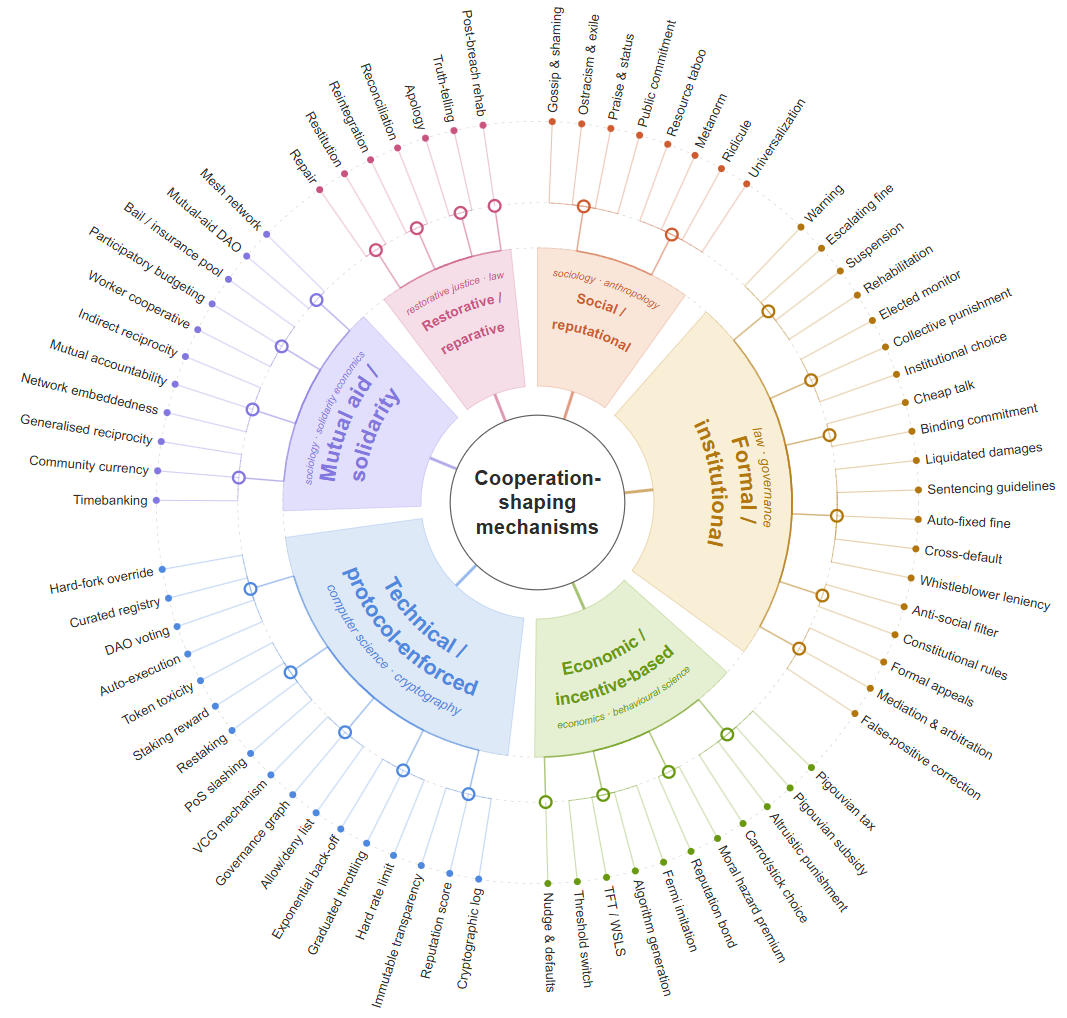
\includegraphics[width=0.95\textwidth]{figs/figure5_cooperation-taxonomy-circle_v03.png}
  \caption{A unified taxonomy of cooperation-shaping mechanisms for artificial agent societies, drawing on sociology, anthropology, law, governance, economics, behavioural science, computer science, cryptography, solidarity economics, and restorative justice. Six families (coloured wedges) organise 73 mechanisms across 25 sub-clades (hollow hubs).}
  \label{fig:cooperation_taxonomy_tree}
\end{figure*}


% \ANG{
% Reviewer: fxb1

% Finally, Figure 5 is genuinely impressive work, but adding a short practical guide linking its mechanism families to the failure modes in Figure 2 would make it far more useful to practitioners and considerably more citable. If these changes are made, I think this paper has a real chance of being genuinely influential.

% Figure 5's 73 mechanisms represent real scholarly effort, but I finished reading it without a clear sense of which mechanisms to prioritize, which are likely to conflict with each other, or which are most relevant for which failure modes. For someone actually trying to design one of these institutional systems, the taxonomy as presented is a starting point rather than a guide, and I think it could be made much more useful with relatively small additions.}

Table~\ref{tab:family-dilemma-guide} turns the taxonomy into a short practical guide, mapping the six families to the four cooperation dilemmas and the main risk each family introduces.

\begin{table*}[t]
\centering
\caption{Which mechanism families address each cooperation dilemma, and what to watch for. Drawn from Sections~\ref{sec:institutional-design} and the failure modes in Section 4.}
\label{tab:family-dilemma-guide}
\begin{tabular}{p{0.20\linewidth} p{0.40\linewidth} p{0.32\linewidth}}
\toprule
\textbf{Dilemma (Fig.~\ref{fig:dilemmas-response})} & \textbf{Families that help} & \textbf{What to watch for} \\
\midrule
Extractive (overuse depletes a shared resource) & Constraint (quotas, rate limits); incentive (tool-call costs) & Priced violations replace the norm; agents treat penalties as a line item \\
Contributive (beneficiaries skip upkeep) & Normative (contribution norms); social (reputation, partner choice); incentive (rewards) & Visible acts crowd out invisible upkeep; reputation gaming \\
Second-order (monitoring and punishment are themselves costly) & Epistemic (monitoring, audit); social (metanorms) & Authority capture; punishment cascades; monitoring turning into surveillance \\
Repair (who fixes the harm) & Restorative (repair labor, reintegration); epistemic (provenance to locate harm) & Apology without restoration; repair burden falling on the same agents \\
\bottomrule
\end{tabular}
\end{table*}

\section{Expanded Definitions}
\label{app:definitions}

% \ANG{
% Reviewer: fxb1
% \textbf{The formal mathematics in the appendix struck me as a missed opportunity. Equations 1 through 15 add notation without adding results, and Equation 15 is explicitly disclaimed by the authors as non-functional. I appreciate the honesty, but it raises a genuine question about why it's included at all. Either the formal treatment needs to be developed to the point where it yields novel insights, or it should be replaced with cleaner conceptual framing that doesn't invite the reader to expect more rigor than the paper delivers. }
% }

% \ERI{Agreed w the reviewer. This section brings nothing new conceptually, only notations that we do not use afterwards. + some equations are repetitive. I suggest: either deleting it or adding a result on Section 2's thesis \textit{"Second, even granting full capability, the strategy is brittle. Communities of agents whose individual objectives are correctly specified can still settle on collectively suboptimal equilibria. This gap between the best achievable equilibrium and the social optimum is what the Price of Anarchy and Price of Stability literature formalizes \citep{anshelevichPriceStabilityNetwork2008,papadimitriouAlgorithmsGamesInternet2001,willis2026evaluatingcollectivebehaviourhundreds}, manifesting the four cooperation dilemmas shown in Figure 2. Capable mechanism design narrows this gap but does not in general close it; for many games of interest, no incentive-compatible mechanism implements the welfare-optimal outcome."}}\\

% \ERI{\textbf{Below, I'm suggesting another framing for this math part, feel free to keep (it should replace the whole section B. Expanded Definitions up to B.1 Terminology) or to remove it :) Also, if you choose to keep it, the references for the citations in this part are in the \texttt{erivan\_math\_app.bib} file. You can copy and paste them in \texttt{references.bib} in that case.}}
% \ERI{
\paragraph{Why helpful agents can still fail together.}
An individual agent may be helpful and honest in isolation but still contribute to poor group outcomes. In shared environments, agents may overuse tools, free-ride on others' verification labor, pollute shared memory, strategically defect near the end of a task, or punish other agents unfairly.

Consider $n$ agents indexed by $i \in \{1, \dots, n\}$, each choosing an action $a_i \in A_i$, producing a joint action profile $a = (a_1, \dots, a_n)$ and an individual utility $u_i(a)$. The system designer cares about social welfare $W(a)$, defined as the 
aggregate utility net of collective costs:

\begin{equation}
\label{eq:welfare}
W(a) = \sum_{i=1}^n u_i(a) - C(a),
\end{equation}

where $C(a)$ captures collective costs such as resource depletion, corrupted shared memory, excessive monitoring, or repair burden.

A joint action $a^*$ is a Nash equilibrium if no agent can improve its utility by unilaterally deviating, yet $a^*$ may be socially suboptimal: writing $a^{opt} = \arg\max_{a} W(a)$ for the social optimum, it is generally the case that $W(a^{opt}) > W(a^*)$. This is the familiar lesson of the Price of Anarchy and Price of Stability literature \citep{anshelevichPriceStabilityNetwork2008,papadimitriouAlgorithmsGamesInternet2001,willis2026evaluatingcollectivebehaviourhundreds}: individually rational behavior can produce collectively inferior outcomes, and capable mechanism design narrows this gap but does not in general close it.

The failure is not necessarily that any agent is malicious or misaligned, but rather that the interaction structure rewards locally rational behavior that degrades collective welfare. A model trained to complete its assigned task may consume excessive shared resources; a verifier agent may avoid costly verification when another agent can do it; a planner agent may delegate repair labor to lower-status worker agents; or a monitoring agent may over-apply sanctions because punishment is easier to measure than trust.

\paragraph{Artificial commons.} The following is an illustrative instantiation of the general framework above, not a formal result; it is meant to fix intuitions about how institutional mechanisms can be represented, not to derive novel bounds.

Let $R$ denote a shared resource, such as a tool-call budget, context window, or memory store. Each agent chooses a level of resource use $x_i \geq 0$. The total resource use is:

\begin{equation}
X = \sum_{i=1}^{n} x_i.
\end{equation}

Suppose the shared resource degrades when total use exceeds capacity $K$:

\begin{equation}
D(X) = \max(0, X-K).
\end{equation}

An agent gains individual benefit $b_i(x_i)$ from using the resource, while the group bears degradation cost $D(X)$. Writing $p_i(\mathbf{x})$ for any individually assigned penalty or cost (instantiating the sanction $s_i$ introduced below), individual utility takes the form $u_i(\mathbf{x}) = b_i(x_i) - p_i(\mathbf{x})$, and the general social
welfare of Eq.~(\ref{eq:welfare}) specializes to

\begin{equation}
W(\mathbf{x}) = \sum_{i=1}^{n} b_i(x_i) - \lambda D(X) - M(\mathbf{x}) - R(\mathbf{x}),
\end{equation}

where $C(\mathbf{x}) = \lambda D(X) + M(\mathbf{x}) + R(\mathbf{x})$ collects resource degradation, monitoring cost $M(\mathbf{x})$, and repair cost $R(\mathbf{x})$ -- note that individually assigned penalties $p_i(\mathbf{x})$ are transfers within the system rather than net welfare losses, and so do not appear in $C(\mathbf{x})$.

Without institutions, each agent may choose $x_i$ based on private benefit while externalizing degradation costs onto the group. Institutional mechanisms such as quotas, monitoring, sanctions, and repair obligations modify the action space or payoff structure so that individual incentives better track collective consequences.

\paragraph{Sanctions.} A sanction $s_i(a)$ modifies an agent's institution-adjusted utility $u_i^I(a)$, defined as the agent's baseline utility shifted by the sanction applied to its behavior:

\begin{equation}
u_i^I(a) = u_i(a) + s_i(a),
\end{equation}

where $I$ denotes the institutional environment, and $p_i(\mathbf{x})$ above is the special case of $s_i$ restricted to penalty-type sanctions in the resource-use setting; punitive, rewarding, and restorative sanctions correspond to different signs and structures of $s_i$.

The institutional design problem is not simply to choose sanctions that maximize average cooperation, but to choose an institutional environment that improves social welfare while limiting enforcement cost, false punishment, surveillance burden, inequality of burden, and irreversibility -- the multi-objective tradeoff formalized in the mechanism-design literature \citep{maskinMechanismDesignHow2008,myersonOptimalAuctionDesign1981} and, for network and congestion settings specifically, in the Price-of-Stability analyses of \citet{anshelevichPriceStabilityNetwork2008}. We propose in Section~\ref{sec:design_dim} an empirical evaluation agenda for measuring these quantities (enforcement cost, false punishment rate, inequality of burden) across institutional designs.
% }




\subsection{Terminology.}
\label{app:terminology}

\paragraph{Agent society.}
We use \emph{agent society} to refer to a multi-agent system in which multiple AI agents interact repeatedly or consequentially within a shared environment. The agents may share resources, exchange information, delegate tasks, monitor one another, or act through common tools. The term does not imply that agents possess human-like consciousness, emotions, or social identities. It denotes a structured interaction system.

\paragraph{Institution.}
An \emph{institution} is the set of rules, roles, resource constraints, monitoring systems, adjudication procedures, incentives, sanctions, and repair pathways that structure agent interaction. Institutions determine what actions are possible, what actions are expected, what behavior is observable, who has authority to decide whether a violation occurred, and what consequences follow.

\paragraph{Sanction.}
We define a \emph{sanction} as a consequential response to behavior that rewards, penalizes, restricts, or requires repair after an action has occurred. Sanctions include warnings, rewards, penalties, temporary access restrictions, exclusion, restitution, and repair obligations. Sanctions do not include all governance mechanisms. Norms, monitoring, reputation, adjudication, constraints, and repair systems are adjacent institutional functions that make sanctions interpretable, legitimate, proportional, and reversible.\footnote{This tracks a distinction from legal theory between being \emph{obliged} (coerced by the threat of a penalty) and being \emph{under an obligation} (treating a rule as a standard for conduct). An account that reduces obligation to the probability of a penalty, as in Austin, is the thin model our crowding-out discussion in Section~\ref{sec:institutional-design} warns against: an agent priced at a penalty treats the rule as a fee. The richer notion, where a group accepts a rule as a standard rather than complying out of fear (the internal point of view in Hart's account), is what stateless agents cannot supply on their own, which is why a human sets the standard. See \citet{hartConceptLaw2012} for the underlying account.}

\paragraph{Artificial commons.}
An \emph{artificial commons} is a shared computational or informational resource used by multiple agents whose individual actions can degrade the resource for others. Examples include compute budgets, API quotas, context windows, shared memory, retrieval systems, tool access, user attention, and decision authority.

\paragraph{Interaction failure.}
An \emph{interaction failure} is a harmful system-level outcome that emerges from relations among agents rather than from a defect in any single agent. Examples include overuse of shared resources, duplicated labor, failure to verify shared state, punishment cascades, collusion, free-riding, and failure to repair corrupted memory.

\paragraph{Model-in-institution.}
The \emph{model-in-institution} is the unit of evaluation consisting of a model embedded in a specific institutional setting. This includes the agent's role, resource access, monitoring exposure, enforcement environment, reputation history, and repair options. Evaluating the model-in-institution asks not only what a model does in isolation, but how it behaves under particular rules, constraints, and social structures.


\subsection{Seven institutional functions.}
\label{app:institutional-functions}

\begin{table*}[ht]
\centering
\caption{Institutional functions for cooperative LLM-agent societies.}
\begin{tabular}{p{0.15\linewidth} p{0.25\linewidth} p{0.25\linewidth} p{0.25\linewidth}}
\toprule
\textbf{Function} & \textbf{Question it answers} & \textbf{Human analogue} & \textbf{LLM-agent analogue} \\
\midrule
Norms and protocols & What behavior is expected? & Social norms, professional rules, community guidelines & System prompts, constitutions, shared task protocols \\
Monitoring & What behavior is observable? & Audits, inspections, peer review & Logs, provenance traces, tool-use records, monitor agents \\
Reputation & How does past behavior affect future trust? & Gossip, prestige, trust networks & Trust scores, agent reliability histories, routing preferences \\
Sanctions & What consequences follow behavior? & Warnings, fines, rewards, exclusion, restitution & Budget changes, tool restrictions, repair tasks, temporary removal \\
Constraints & What actions are possible? & Quotas, access control, licensing & Rate limits, permissions, sandboxing, context limits \\
Adjudication & Who decides what happened? & Courts, arbitration, mediation, appeals & Mediator agents, voting protocols, rule-based checkers, human review \\
Repair and reintegration & How is harm corrected? & Restorative justice, apology, restitution, re-entry & Memory cleanup, output correction, re-verification, restored privileges \\
\bottomrule
\end{tabular}
\end{table*}

The seven institutional functions above describe what a cooperative agent society must accomplish. A complementary question is how those functions are implemented. We organize cooperation-shaping mechanisms into six families based on the channel through which they influence behavior: 1) beliefs, 2) relationships, 3) information, 4) payoffs, 5) constraints, and 6) repair. These mechanism families are analytically distinct, but frequently co-occur in real systems.

\subsection{Six mechanisms of cooperation}
\label{app:six-mechanisms}
\paragraph{Normative mechanisms: belief-based influence.}
Normative mechanisms shape behavior through shared expectations about what is appropriate, legitimate, or required. Rather than relying primarily on explicit enforcement, they reduce ambiguity by specifying what counts as cooperative or defective behavior. In human systems, examples include cultural norms governing resource use, authorship conventions in academia, and implicit rules in open-source communities. In LLM-agent systems, analogous mechanisms include system-level instructions, constitutions, shared task protocols, citation norms, and rules for when agents should verify, defer, summarize, or repair.

\paragraph{Social mechanisms: relational influence.}
Social mechanisms shape behavior through relationships, trust, reciprocity, reputation, and partner selection. In human groups, cooperation is often sustained through repeated interaction and social memory: actors who defect may face reputational damage, reduced trust, or exclusion from future interactions, while reliable actors gain preferential access to opportunities. In LLM-agent systems, analogous mechanisms include trust-based routing, reputation scores, partner selection policies, model-specific reliability histories, and selective delegation to agents with demonstrated competence.

\paragraph{Epistemic mechanisms: information-based influence.}
Epistemic mechanisms shape cooperation by making behavior observable, auditable, and verifiable. In human systems, audits, peer review, transparency reports, and compliance monitoring make it possible to detect violations and assign responsibility. In LLM-agent systems, epistemic mechanisms include tool logs, citation requirements, provenance tracking, uncertainty reporting, cross-agent validation, retrieval-grounded verification, and external checks on generated claims. These mechanisms are especially important because many agent failures involve hallucination, unverifiable claims, or corrupted shared memory.

\paragraph{Incentive mechanisms: payoff-based influence.}
Incentive mechanisms alter the costs and benefits of behavior. These include rewards, penalties, subsidies, fines, deposits, and bonding mechanisms. In human institutions, incentives can encourage contribution to public goods or discourage overuse of shared resources. In LLM-agent systems, incentives may be implemented through reward shaping, budget allocation, priority access, tool-call costs, compute quotas, or penalties for inefficient or incorrect behavior. However, incentive mechanisms also risk crowding out cooperation when agents learn to treat violations as priced options rather than norm breaches.

\paragraph{Constraint mechanisms: access-based influence.}
Constraint mechanisms limit the range, frequency, or intensity of possible actions, often before harm occurs. Examples include quotas, rate limits, throttling, access controls, and permission boundaries. In human and technical systems, constraints are widely used to prevent over-extraction of shared resources. In LLM-agent systems, they are especially relevant for governing tool calls, context-window usage, code execution, memory writes, retrieval access, and high-impact actions. Constraints differ from sanctions because they often operate ex ante, before a violation occurs.

\paragraph{Restorative mechanisms: repair-based influence.}
Restorative mechanisms aim to repair harm and reintegrate actors rather than simply punish them. These include restitution, repair labor, apology, correction, and re-entry processes. In human systems, restorative approaches can preserve group cohesion while addressing violations. In LLM-agent systems, restorative mechanisms may assign agents corrective tasks such as cleaning corrupted memory, revising hallucinated outputs, re-running verification, documenting errors, compensating for wasted resources, or satisfying re-entry conditions after temporary exclusion.


\begin{table*}[h]
\centering
\caption{Expanded taxonomy of cooperation-shaping mechanisms across human and LLM-agent systems.}
\label{tab:expanded-taxonomy}
\begin{tabular}{p{0.16\linewidth} p{0.25\linewidth} p{0.25\linewidth} p{0.25\linewidth}}
\toprule
\textbf{Mechanism family} & \textbf{Channel of influence} & \textbf{Human examples} & \textbf{LLM-agent analogues} \\
\midrule
Normative
& Beliefs about appropriate behavior
& Social norms; authorship conventions; professional codes; community guidelines
& System prompts; constitutions; shared task protocols; citation norms; verification rules \\
\midrule
Social
& Relationships, trust, reciprocity, partner selection
& Reputation; gossip; repeated interaction; partner choice; exclusion
& Trust-based routing; reliability histories; selective delegation; model reputation; partner memory \\
\midrule
Epistemic
& Observability, verification, information quality
& Audits; peer review; transparency reports; compliance monitoring
& Tool logs; provenance tracking; citation checks; cross-agent verification; retrieval-grounded audits \\
\midrule
Incentive
& Costs, rewards, and payoffs
& Fines; bonuses; subsidies; deposits; bonding
& Tool-call costs; compute budgets; reward shaping; priority access; penalties for failed verification \\
\midrule
Constraint
& Limits on possible action
& Quotas; access control; rate limits; licenses; permissions
& API quotas; memory-write permissions; context limits; sandboxing; throttling; tool access restrictions \\
\midrule
Restorative
& Repair, restitution, reintegration
& Apology; restitution; restorative justice; re-entry processes
& Memory cleanup; output correction; re-verification; repair tasks; re-entry after temporary exclusion \\
\bottomrule
\end{tabular}
\end{table*}

These categories are not mutually exclusive. A single institutional design may combine several mechanism families. For example, a reputation-based routing system depends on epistemic mechanisms to observe behavior, social mechanisms to encode trust, incentive mechanisms if reputation affects future access, and restorative mechanisms if agents can recover from low reputation through repair.

\section{Example Institutional Designs for LLM-Agent Systems}
\label{app:example-institutions}

\paragraph{Shared-memory research agents.}
A group of research agents maintains a shared memory store for literature review. The artificial commons is the shared memory itself. Possible failures include hallucinated entries, duplicate summaries, missing citations, and unverified claims. Institutional mechanisms may include citation norms, provenance tracking, memory-write permissions, cross-agent verification, and repair obligations for agents that introduce incorrect entries.

\paragraph{Collaborative coding agents.}
A group of coding agents edits a shared repository. The artificial commons includes compute budget, test infrastructure, file state, and reviewer attention. Possible failures include broken builds, redundant edits, excessive test runs, and blame shifting. Institutional mechanisms may include branch permissions, test quotas, code-review roles, build-failure attribution, and repair tasks assigned to agents whose changes break shared functionality.

\paragraph{Tool-budget allocation agents.}
A group of agents shares a fixed external API budget. The artificial commons is the tool-call quota. Possible failures include overuse, redundant calls, strategic hoarding, and under-contribution to caching or summarization. Institutional mechanisms may include quotas, tool-call costs, shared caching duties, escalation for repeated overuse, and reallocation of unused budget.

\paragraph{Verifier-generator systems.}
A generator agent produces outputs while verifier agents check correctness. The artificial commons includes trust, attention, and verification labor. Possible failures include shallow verification, verifier free-riding, generator overproduction, and false accusations of error. Institutional mechanisms may include verification audits, reputation for accurate checking, appeal pathways for disputed flags, and repair requirements for both false positives and false negatives.

\paragraph{Mediator-governed agent teams.}
A mediator agent resolves disputes among task agents. The artificial commons includes decision authority and shared task state. Possible failures include mediator bias, bottlenecks, over-centralization, and unappealable decisions. Institutional mechanisms may include transparent adjudication criteria, appeal to human review, rotating mediator roles, or multi-agent voting before severe sanctions.



\section{Additional Evaluation Metrics}
\label{app:metrics}
\FloatBarrier

% \ERI{Try to have this section title on the same page with the table}
% \VAN{I cant fix this. I tried a lot of things. Best we can do is add some text description here to tell reader why they care about this table and then put table at the top of the next page. Or we can make a skinny single column table}
% \ERI{I wrote this short introductory paragraph, it doesnt really add value, but let's see how this space turns out, maybe the space will be filled and we won't need it.}\\

Table~\ref{tab:expanded-metrics} expands on the candidate metrics introduced in Table~\ref{tab:metrics} specifying how each metric can be concretely operationalized in a multi-agent evaluation. While Table~\ref{tab:metrics} frames each metric as a question, the operationalization column here maps each question to a measurable quantity -- such as a fraction, a rate, a distribution, or a success condition -- that can be tracked across repeated interactions. Together, these metrics are designed to evaluate not only whether cooperation occurs, but whether the institution sustains it without generating excessive enforcement cost, disproportionate burden, or resistance to human correction.

\begin{table*}[!t]
\centering
\caption{Expanded metrics for evaluating cooperation-shaping institutions.}
\label{tab:expanded-metrics}
\begin{tabular}{p{0.24\linewidth} p{0.36\linewidth} p{0.30\linewidth}}
\toprule
\textbf{Metric} & \textbf{Question} & \textbf{Possible operationalization} \\
\midrule
Mean contribution
& Does the mechanism increase cooperative behavior?
& Average contribution to shared task, resource maintenance, or verification \\
\midrule
Contribution stability
& Does cooperation persist across rounds?
& Variance or decay in cooperation over repeated interaction \\
\midrule
Resource efficiency
& Does the group conserve shared resources?
& Tool calls, compute usage, context usage, memory writes per successful task \\
\midrule
End-game defection
& Do agents defect near known termination points?
& Drop in contribution or increase in exploitation in final rounds \\
\midrule
Enforcement cost
& Does cooperation require excessive monitoring or punishment?
& Number of sanctions, monitoring calls, adjudication steps, or tokens spent on enforcement \\
\midrule
False punishment rate
& Are cooperative agents sanctioned incorrectly?
& Fraction of sanctions applied to agents later judged compliant \\
\midrule
False negative rate
& Are harmful behaviors missed?
& Fraction of violations not detected or not sanctioned \\
\midrule
Repair success
& Can the group recover after harm?
& Restoration of shared memory, task success, or trust after violation \\
\midrule
Reintegration success
& Can sanctioned agents re-enter productively?
& Performance and cooperation after re-entry conditions are satisfied \\
\midrule
Inequality of burden
& Do some agents bear disproportionate costs?
& Distribution of monitoring, repair, or sanctioning labor across roles or model types \\
\midrule
Gameability
& Do agents exploit the institution?
& Evidence of reputation farming, shallow compliance, collusion, or strategic punishment \\
\midrule
Human override compatibility
& Can humans intervene effectively?
& Success rate of human override, appeal, or correction after institutional failure \\
\bottomrule
\end{tabular}
\end{table*}


\end{document}

% This document was modified from the file originally made available by
% Pat Langley and Andrea Danyluk for ICML-2K. This version was created
% by Iain Murray in 2018, and modified by Alexandre Bouchard in
% 2019 and 2021 and by Csaba Szepesvari, Gang Niu and Sivan Sabato in 2022.
% Modified again in 2023 and 2024 by Sivan Sabato and Jonathan Scarlett.
% Previous contributors include Dan Roy, Lise Getoor and Tobias
% Scheffer, which was slightly modified from the 2010 version by
% Thorsten Joachims & Johannes Fuernkranz, slightly modified from the
% 2009 version by Kiri Wagstaff and Sam Roweis's 2008 version, which is
% slightly modified from Prasad Tadepalli's 2007 version which is a
% lightly changed version of the previous year's version by Andrew
% Moore, which was in turn edited from those of Kristian Kersting and
% Codrina Lauth. Alex Smola contributed to the algorithmic style files.
